\documentclass[a4paper]{article}

\RequirePackage[undo-recent-deprecations]{expl3} %% Fix: latex3 problem with ebproof

\usepackage[pages=all, color=black, position={current page.south}, placement=bottom, scale=1, opacity=1, vshift=5mm]{background}
%% \SetBgContents{
%% 	\tt This work is shared under a \href{https://creativecommons.org/licenses/by-sa/4.0/}{CC BY-SA 4.0 license} unless otherwise noted
%% }      % copyright

\usepackage[margin=1in]{geometry} % full-width

% AMS Packages
\usepackage{amsmath}
\usepackage{amsthm}
\usepackage{amssymb}

% Unicode
\usepackage[utf8]{inputenc}
\usepackage{hyperref}
\hypersetup{
	unicode,
%	colorlinks,
%	breaklinks,
%	urlcolor=cyan,
%	linkcolor=blue,
	pdfauthor={Author One, Author Two, Author Three},
	pdftitle={A simple article template},
	pdfsubject={A simple article template},
	pdfkeywords={article, template, simple},
	pdfproducer={LaTeX},
	pdfcreator={pdflatex}
}

% Vietnamese
%\usepackage{vntex}

% Natbib
\usepackage[sort&compress,numbers,square]{natbib}
%\bibliographystyle{mplainnat}
\bibliographystyle{plain}

% Theorem, Lemma, etc
\theoremstyle{plain}
\newtheorem{theorem}{Theorem}
\newtheorem{corollary}[theorem]{Corollary}
\newtheorem{lemma}[theorem]{Lemma}
\newtheorem{claim}{Claim}[theorem]
\newtheorem{axiom}[theorem]{Axiom}
\newtheorem{conjecture}[theorem]{Conjecture}
\newtheorem{fact}[theorem]{Fact}
\newtheorem{hypothesis}[theorem]{Hypothesis}
\newtheorem{assumption}[theorem]{Assumption}
\newtheorem{proposition}[theorem]{Proposition}
\newtheorem{criterion}[theorem]{Criterion}
\theoremstyle{definition}
\newtheorem{definition}[theorem]{Definition}
\newtheorem{example}[theorem]{Example}
\newtheorem{remark}[theorem]{Remark}
\newtheorem{problem}[theorem]{Problem}
\newtheorem{principle}[theorem]{Principle}

%%% ebproof column width
\newcommand{\rulewidth}{.8\linewidth}
\newcommand{\ruleverticalsephalf}{0.25cm}
\newcommand{\ruleverticalsep}{0.5cm}

\usepackage{graphicx, color}
\graphicspath{{fig/}}

%\usepackage[linesnumbered,ruled,vlined,commentsnumbered]{algorithm2e} % use algorithm2e for typesetting algorithms
\usepackage{algorithm, algpseudocode} % use algorithm and algorithmicx for typesetting algorithms
\usepackage{mathrsfs} % for \mathscr command

\usepackage{lipsum}

%%% RPC Calculi related commands %%%

%%
\usepackage{listings}
\lstset
{
    basicstyle=\footnotesize\ttfamily,
    numbers=left,
    stepnumber=1,
    frame=single,
}
\usepackage{ebproof}
\usepackage{multicol}
\usepackage{xspace}
\usepackage{stmaryrd} % \llbracket \rrbracket

%% Macros for General Inference Rules
\newcommand{\rpc}{$\lambda_{rpc}$\xspace}
\newcommand{\typedrpc}{$\lambda_{rpc}^{typed}$\xspace}
\newcommand{\polyrpc}{$\lambda_{rpc}^{\forall}$\xspace}
\newcommand{\polyrpcM}{$\lambda_{rpc}^{\forall,M}$\xspace}
\newcommand{\polyrpcA}{$\lambda_{rpc}^{\forall,@}$\xspace}
\newcommand{\linksrpc}{$\lambda_{rpc}^{Links}$\xspace}
\newcommand{\kindedpolyrpc}{$\lambda_{rpc}^{\forall,k}$\xspace}

\newcommand{\stateencrpc}{$\lambda_{rpc}^{enc}$\xspace}
\newcommand{\statefulrpc}{$\lambda_{rpc}^{state}$\xspace}

\newcommand{\cs}{$\lambda_{cs}$\xspace}
\newcommand{\polycs}{$\lambda_{cs}^{\forall}$\xspace}
\newcommand{\stateenccs}{$\lambda_{cs}^{enc}$\xspace}
\newcommand{\statefulcs}{$\lambda_{cs}^{state}$\xpace}

\newcommand{\client}{\textbf{c}}
\newcommand{\server}{\textbf{s}}
\newcommand{\clientserver}{\textbf{cs}}

\newcommand{\statickind}{sta}
\newcommand{\dynamickind}{dyn}

\newcommand{\evalRPC}[3]{#1\Downarrow_{#2}#3}
\newcommand{\evalRPCC}[2]{#1\Downarrow_{\client}#2}
\newcommand{\evalRPCS}[2]{#1\Downarrow_{\server}#2}
\newcommand{\lamL}[3]{\lambda^{#1}#2.#3}
\newcommand{\appL}[3]{#1{\ }^{#2}#3}
\newcommand{\subst}[2]{\{#1/#2\}}
\newcommand{\llet}[3]{\textsf{let} \ #1 = #2 \ \textsf{in} \ #3}
\newcommand{\ldokeyword}{\textsf{do}}
\newcommand{\ldo}[3]{\textsf{do} \ #1 \leftarrow #2 \ \textsf{in} \ #3}
\newcommand{\ldovoid}[2]{\textsf{do} \ #1 \ \textsf{in} \ #2}
\newcommand{\lunit}[1]{\textsf{unit} \ #1}

\newcommand{\textsfGen}{\textsf{gen}}
\newcommand{\gen}[3]{\textsfGen(#1,#2,#3)}

\newcommand{\textsfReq}{\textsf{req}}
\newcommand{\req}[2]{\textsfReq(#1,#2)}

\newcommand{\textsfCall}{\textsf{call}}
\newcommand{\call}[2]{\textsfCall(#1,#2)}

\newcommand{\textsfRet}{\textsf{ret}}
\newcommand{\ret}[1]{\textsfRet(#1)}

\newcommand{\textsfCase}{\textsf{case}}
\newcommand{\textsfOf}{\textsf{of}}
\newcommand{\case}[2]{\textsfCase ~ #1 ~\textsfOf ~ #2}

\newcommand{\fun}{\rightarrow}
\newcommand{\funL}[1]{\xrightarrow{#1}}
\newcommand{\funLC}[2]{\xrightarrow[#2]{#1}}
\newcommand{\tyenv}{\Gamma}
\newcommand{\tyenvExt}[2]{\Gamma,#1:#2}
\newcommand{\tyenvExtWith}[1]{\Gamma,#1}
\newcommand{\varenv}{\Delta}
\newcommand{\varenvExt}[1]{\Delta,#1}
%\newcommand{\typing}[4]{#1\rhd_{#2} #3 : #4}
\newcommand{\typing}[4]{#1\vdash_{#2} #3 : #4}
\newcommand{\kinding}[3]{#1\vdash #2 : #3}
\newcommand{\funtyping}[5]{#1\vdash #4 : #5}     % ;#2, #3
\newcommand{\codetyping}[4]{#1\vdash_{code} #3 : #4}  % _{#2}
\newcommand{\polytyping}[5]{#1;#2\vdash_{#3} #4 : #5}
\newcommand{\conftyping}[2]{\vdash #1 : #2}
\newcommand{\stacktyping}[3]{\vdash_{#1} #2 : #3}
\newcommand{\fvtyping}[2]{#1\vdash #2}

\newcommand{\typingBlack}[4]{#1\blacktriangleright_{#2} #3 : #4}

\newcommand{\loceta}[2]{{#1}\rightsquigarrow{#2}}

\newcommand{\enc}{\textsf{enc}}
\newcommand{\evalStateEncRPCC}[2]{$#1\Downarrow_{\client}^{\enc}#2$}
\newcommand{\evalStateEncRPCS}[3]{$#1;#2\Downarrow_{\server}^{\enc}#3$}

\newcommand{\sta}{\textsf{state}}
\newcommand{\evalStatefulRPCC}[3]{\evalStatefulRPC{#1}{#2}{\client}{#3}}
\newcommand{\evalStatefulRPCS}[3]{\evalStatefulRPC{#1}{#2}{\server}{#3}}
\newcommand{\evalStatefulRPC}[4]{${#1};{#2}\Downarrow_{#3}^{\sta}{#4}$}

\newcommand{\deep}{\textsf{deep}}
\newcommand{\evalDeeplyStatefulRPCC}[3]{\evalDeeplyStatefulRPC{#1}{#2}{\client}{#3}}
\newcommand{\evalDeeplyStatefulRPCS}[3]{\evalDeeplyStatefulRPC{#1}{#2}{\server}{#3}}
\newcommand{\evalDeeplyStatefulRPC}[4]{${#1};{#2}\Downarrow_{#3}^{\deep}{#4}$}

\newcommand{\IdK}{\textsf{Id}}
\newcommand{\FunK}[3]{\textsf{Fun} \ #2 \ #3}
\newcommand{\AppK}[3]{\textsf{App} \ #2 \ #3}
%\newcommand{\FunK}[3]{\textsf{Fun}^{#1} \ #2 \ #3}
%\newcommand{\AppK}[3]{\textsf{App}^{#1} \ #2 \ #3}

\newcommand{\reify}[1]{\ulcorner #1 \urcorner}

\newcommand{\RightarrowEnc}{\Rightarrow^{enc}}
\newcommand{\RightarrowEncStar}{\Rightarrow^{enc*}}
\newcommand{\RightarrowEncPlus}{\Rightarrow^{enc+}}

\newcommand{\runStateEncRPC}[2]{$#1 \RightarrowEnc #2$}
\newcommand{\runStateEncRPCStar}[2]{$#1 \RightarrowEncStar #2$}
\newcommand{\runStateEncRPCPlus}[2]{$#1 \RightarrowEncPlus #2$}

\newcommand{\runStateEncCS}[2]{$#1 \Rightarrow^{enc} #2$}
\newcommand{\runStateEncCSStar}[2]{$#1 \Rightarrow^{enc*} #2$}

\newcommand{\runStatefulRPC}[2]{$#1 \Rightarrow^{state} #2$}
\newcommand{\runStatefulRPCStar}[2]{$#1 \Rightarrow^{state*} #2$}

\newcommand{\runStatefulCS}[2]{$#1 \Rightarrow^{state} #2$}
\newcommand{\runStatefulCSStar}[2]{$#1 \Rightarrow^{state*} #2$}

\newcommand{\emp}{\epsilon}
\newcommand{\substzsxs}{\{\bar{v}/\bar{z},\overline{w}/\bar{x} \}}
\newcommand{\substxs}{\{\overline{w}/\bar{x} \}}

\newcommand{\substZsXs}{\{\overline{V}/\bar{z},\overline{W}/\bar{x} \}}
\newcommand{\substXs}{\{\overline{W}/\bar{x} \}}

\newcommand{\LetK}[2]{\textsf{ctx}\ #1 \ #2}
%\newcommand{\LetK}[2]{(#1,#2)}
\newcommand{\opt}[1]{#1_{opt}}

\newcommand{\overlineK}{\overline{K}}
\newcommand{\overlinePi}{\overline{\Pi}}
\newcommand{\overlineDelta}{\overline{\Delta}}

%\newcommand{\comp}[1]{\rightsquigarrow_{#1}}
%\newcommand{\comps}{\rightsquigarrow_{\server}}
%\newcommand{\compc}{\rightsquigarrow_{\client}}
% \newcommand{\ccomp}[1]{\mathcal{C}[\![#1]\!]}
\newcommand{\ccomp}[1]{\mathcal{C}\llbracket#1\rrbracket}
%\newcommand{\scomp}[1]{S[\![#1]\!]}
% \newcommand{\vcomp}[1]{\mathcal{V}[\![#1]\!]}
\newcommand{\vcomp}[1]{\mathcal{V}\llbracket#1\rrbracket}
%\newcommand{\cconv}[1]{CC[\![#1]\!]}
%\newcommand{\cconvprg}[1]{CC_{prg}[\![#1]\!]}
\newcommand{\typeinf}[1]{G[\![#1]\!]}

% \newcommand{\ecomp}[1]{[\![#1]\!]}
\newcommand{\ecomp}[1]{\llbracket#1\rrbracket}

\newcommand{\linkstycomp}[2]{\llbracket#1\rrbracket_{#2}}
\newcommand{\adjcomp}[4]{#1:#2 \Rightarrow #3:#4}
\newcommand{\judgcomp}[2]{\llbracket#1\rrbracket_{#2}}

\newcommand{\loctycomp}[1]{L\llbracket#1\rrbracket}
\newcommand{\polytycomp}[1]{T\llbracket#1\rrbracket}

\newcommand{\anncomp}[1]{Ann\llbracket#1\rrbracket}
\newcommand{\loctmcomp}[1]{\llbracket#1\rrbracket}


\newcommand{\FUNS}{\Phi}
\newcommand{\funstore}{\FUNS}
\newcommand{\funtype}{\funstore_{type}}
\newcommand{\funcode}{\funstore}
\newcommand{\fv}[1]{\textsf{fv}(#1)}
\newcommand{\dom}[1]{\textsf{dom}(#1)}
\newcommand{\clo}[2]{clo({#1},{#2})}
\newcommand{\cloty}[1]{Clo(#1)}
\newcommand{\valty}[1]{relocatable(#1)}

\newcommand{\Loc}{Loc}

\newcommand{\sessionNothing}{\makebox[0.3cm][c]{\scriptsize $nothing$}}
\newcommand{\sessionSomething}{\makebox[0.3cm][c]{\scriptsize $session$}}
\newcommand{\sessionOption}{\makebox[0.3cm][c]{\scriptsize $optSession$}}

\newcommand{\mono}[1]{[\![#1]\!]}

\newcommand{\optrpc}[1]{\mathcal{O}[\![#1]\!]}

\newcommand{\resolve}[2]{\{\!\{#1\}\!\}^{#2}}

\newcommand{\stack}{\Delta}
\newcommand{\emptystack}{\epsilon}

\newcommand{\conf}{\Sigma}
\newcommand{\confcs}[2]{\langle #1 | #2 \rangle}
\newcommand{\stackcsWith}[2]{ #1  |  #2 }
\newcommand{\stackcs}{\stackcsWith{ \stack_\client }{ \stack_\server }}
\newcommand{\confuntyped}{\sigma}

\newcommand{\run}{\longrightarrow}
\newcommand{\runequiv}{\Longrightarrow}
\newcommand{\structeqv}{\equiv}

\newcommand{\loctyvars}{\overline{l} \ \overline{\alpha}}
\newcommand{\loctys}{\overline{\Loc}\ \overline{A}}

\newcommand{\CloCodeType}{Ty}
\newcommand{\CloCode}{Code}
\newcommand{\OpenCode}{OpenCode}

\newcommand{\at}[1]{@#1}
\newcommand{\eff}{\mbox{\texttt{ctx}}}

\newcommand{\logicalRelText}{R}
\newcommand{\logicalRel}[2]{\logicalRelText \ #1 \ #2}
\newcommand{\logicalRelJudg}[2]{\logicalRelText \ (#1) \ (#2)}
%%%%%%%%%%%%%%%%%%%%%%%%%%%%%%%%%%%%



% Author info
\title{On Static Location in Links\\(A progress report)}
\author{Kwanghoon Choi}
%\author{Author One$^1$\thanks{Author One was partially supported by Grant XXX} \and Author Two$^2$ \and Author Three$^1$}

\date{
  Chonnam National University, Gwangju, Republic of Korea
  \\ \texttt{kwanghoon.choi@jnu.ac.kr}\\[2ex]%
	%% $^1$Organization 1 \\ \texttt{\{auth1, auth3\}@org1.edu}\\%
	%% $^2$Organization 2 \\ \texttt{auth3@inst2.edu}\\[2ex]%
%	\today
}

\begin{document}

\maketitle

\begin{abstract}
%
This progress report describes an attempt to recover static location
contexts in the Links-RPC calculus, which captures the RPC aspect of
Links, by compiling to the polymorphic RPC calculus and back to
itself.
%
Currently, the proposed idea is limited to the rank-1 subset of the
Links-RPC calculus.
%
The limitation is caused by a technical problem involving polymorphic
constructs in the adjustment of locations to resolve the location
discrepancies resulting from our heuristic type compilation.
%
We will continue to study to extend the applicability to the whole
calculus by solving this problem.

\noindent\textbf{Keywords:} Location inference, Links, RPC calculus
\end{abstract}

%\tableofcontents

\section{Introduction}
\label{sec:intro}

A motivation is this.
%
The feature of location types would be good for multi-tier programming
languages like Links in local computation optimization and static
location inconsistency checking.

%
% Examples to explain the two benefits.

%
However, a naive integration of this feature in Links should be
challenging because there might be a need to change several advanced
features in a significant way.
%
An alternative direction would pursue a way to recover static location
contexts in Links equally useful for the aforementioned benefits but
in the hope of no change or minimal changes that do not affect the
Links language system so much.

%
Note that this paper refers to Links as its intermediate
representation, the Links IR.

%
Figure~\ref{fig:addingstaticlocationcontexts} shows a general
methodology to approach this alternative direction by analyzing static
location contexts via compiling to the polymorphic RPC calculus and
then by representing the analyzed context information in Links via
compiling back.

\begin{figure}[ht]
        \centering
        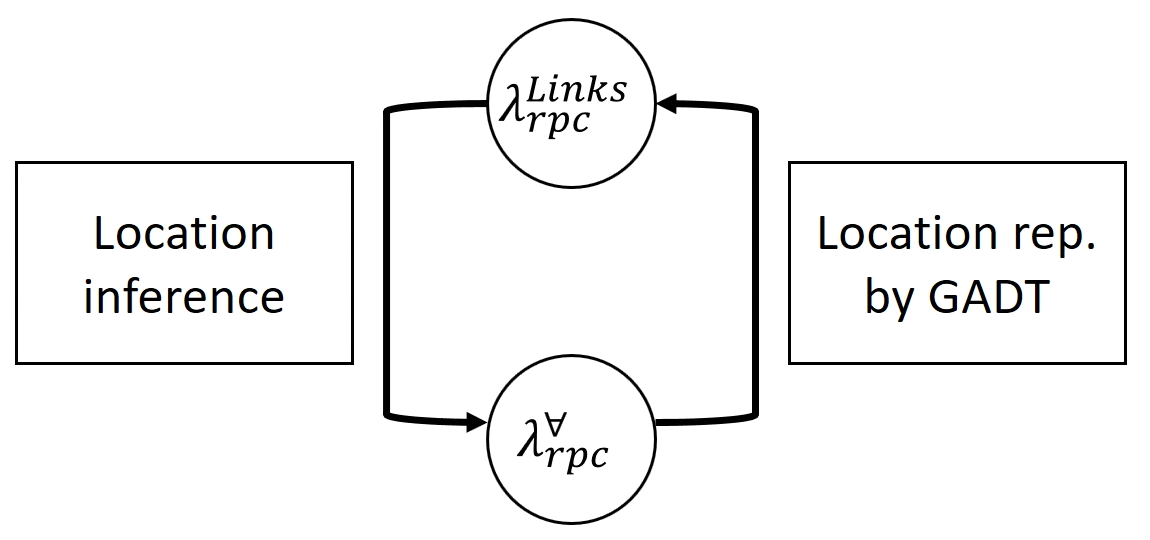
\includegraphics[width=0.6\textwidth]{linksrpc.png}
        \caption{Recovering static location contexts by compiling
          to the polymorphic RPC calculus and back}
        \label{fig:addingstaticlocationcontexts}
\end{figure}

%
Let us discuss location inference and representation by compiling to
the polymorphic RPC calculus and subsequently compiling back.
%
In Links, a client map function would be written as follows.
%

\begin{lstlisting}
  sig map : (a -> b, [a]) -> [b]
  fun map(f, xs) client {
    switch( xs ) {
      case [] -> []
      case y::ys -> f(y) :: map (f, ys)
    }
  }
\end{lstlisting}

%
As seen in the example, having a client location annotation enforces
the map function to run at the client, but the location information is
disregarded by types.
%
Programmers may view the argument type as a client function type of $a
\rightarrow b$ but the client map function could be applied to a
server function of the same type.
%
Therefore, the implementation of $f(y)$ should always check the
location of the function $f$ before its application to $y$.

%
A heuristic could be made up to reflect the programmers' view: by the
presence of the client location annotation, all function types
occurring in the map function type would be assumed to have the same
location annotation.
%
The following signature would describes the idea of this heuristic if
Links did allow such a function type.
%
For notation, $a \funL{client} b$ intends to mean a type of functions
that are guaranteed to run in the client as in the polymorphic RPC
calculus \cite{CHOI:scp2020}.

\begin{lstlisting}
  sig map : (a -client-> b, [a]) -client-> [b]
\end{lstlisting}

A client map function of this imaginary signature might not have to
check the location of the function $f$ in $f(y)$ anymore as long as $f$ is
guaranteed to be a client function as the signature. This is a local computation
optimization.

When the map function is applied to a server function $g$ of type
$a\funL{server}b$, the location of $g$ is required to be adjusted in
some way to run this function inside the client map function that does
not runtime checking.
%
Choi and Chang \cite{choijfp2019} proposed an idea of using an eta
conversion for the location adjustment as
%
\[
fun \ (x) \ client \ { \ g(x) \ }
\]
%
in the Links syntax\footnote{Actually, Links does not allow anonymous
  functions to have location annotations.}.
%
This anonymous function is of type $a\funL{client} b$ as the
signature.
%
It would be responsible for moving to the server to perform the
application of $g(x)$ while the map function is still running in the
client without runtime location checking.

Thus our type inference strategy will consist of a heuristic of
interpreting location annotation as explained and an adjustment of
locations as the eta conversion in the example.


Generally, the map function is written as a location-neutral one where
it should be able to run both of in the client and in the server.
%
In Links, the map function is written without location annotation as
follows.

\begin{lstlisting}
  sig map : (a -> b, [a]) -> [b]
  fun map(f, xs) {
    switch( xs ) {
      case [] -> []
      case y::ys -> f(y) :: map (f, ys)
    }
  }
\end{lstlisting}

%
Programmers could view this unannotated function as a polymorphic
location function.
%
This perception would be made use of when compiling into the
polymorphic RPC calculus where programmers can write location
abstractions and applications with location variables.
%
Combining the previous heuristic with a location variable, a map
function could be made up as a location polymorphic version where $map
\ [client]$ is a client one and $map \ [server]$ is a server one.

\begin{lstlisting}
  sig map : forall l. (a -l-> b, [a]) -l-> [b]
\end{lstlisting}

%
Unfortunately, Links does not support the notion of location variables
nor location abstractions and applications.
%
So, we need to encode this location polymorphism in a way.

%
One way of encoding locations in Links would make use of GADTs as
proposed in Choi et al \cite{CHOI:scp2020}.
%
Firstly, let $Location \ \alpha$ be a GADT whose data constructors are
$Client$ and $Server$.
%
They have type $Location \ ClientType$ and
$Location \ ServerType$, respectively.
%
The polymorphic map function of the signature would be written in
Links, as follows.

\begin{lstlisting}
  sig map : Location l -> (a -> b, [a]) -> [b]
  fun map(z) {
    fun map'(f, xs) {
      switch( xs ) {
        case [] -> []
        case y::ys -> f(y) :: map' (f, ys)
    }
  }
\end{lstlisting}

%
The Links signaure should be interpreted similarly as explained with
the heuristic previously.
%
That is, it would be viewed as $(a \funL{l} b, [a]) \funL{l} [b]$.
%

This polymorphic map function can run wherever it chooses to run by
$map \ Client$ or $map \ Server$ by applying it to one of the data
constructors that represent client and server locations.
%
Interestingly, the polymorphic map function can still run as a local
computation.
%
So, there is no need to refer to $z$ in the map example.

However, in other examples,there is sometimes a need to check
locations in runtime.
%
For this purpose, the polymorphic map function is written to take a
value for representing locations as an argument.
%
When runtime location checking is necessary, the argument $z$ could be
examined.
%

%
This is a glimpse of an idea of location representation when
compiling back to Links.

%% \begin{table}[ht]
%% 	\centering
%% 	\begin{tabular}{|c|c|}
%% 		\hline
%% 		\textbf{Odd} & \textbf{Even} \\
%% 		\hline\hline
%% 		One & Two \\
%% 		\hline
%% 		Three & Four \\
%% 		\hline
%% 	\end{tabular}
%% 	\caption{This is a table}
%% 	\label{tbl:1}
%% \end{table}

%% Table~\ref*{tbl:1} is an example of a table.

%
Section \ref{sec:linksrpc} defines a Links-RPC calculus.
%
Section \ref{sec:translationtopolyrpc} discusses a compilation method
of \polyrpc into \linksrpc.
%
Section \ref{sec:compilationwithgadts} discusses a reverse direction
compilation method.
%
Section \ref{sec:conclusion} concludes.

\section{A Links-RPC Calculus}
\label{sec:linksrpc}

This section describes a RPC calculus that extends the RPC calculus
\cite{Cooper:2009:RC:1599410.1599439} with unannotated
$\lambda$-abstractions whose locations are not specified.
%
The extended RPC calculus intends to capture the RPC feature of the
Links programming language \cite{Cooper:2006:LWP:1777707.1777724} in a
simple way.
%
For our setting, the calculus is also extended with polymorphic types
with type abstractions and applications.
%
Let us call it a Links-RPC calculus, \linksrpc.


\begin{figure}[h]
\centering
\begin{tabular}{ l  l  r  c  l }
\multicolumn{5}{l}{\textbf{Syntax}} \\
 & Location & $a,b$   & $::=$ & $\client \ \ | \  \  \server$ \\
 &          & $?a$    & $::=$  & $a  \ \ |  \ \ (unknown) $ \\
 & Term     & $L,M,N$ & $::=$  & $V  \ | \  L \ M  \ | \  M[A]  \ | \  (L,M)  \ |  \ \pi_i(M)$ \\
 & Value & $V,W$ & $::=$ & $x  \ \ |  \ \ \lambda^{?a} x.M  \ \ |  \ \ \Lambda\alpha.V  \ \ |  \ \ (V,W)$
\\[\ruleverticalsep]
\multicolumn{5}{l}{\textbf{Types}} \\
& Type & $A,B,C$ & $::=$
& $base  \ \ | \ \  A \rightarrow B  \ \ | \ \  \alpha  \ \ | \ \  A \times B  \ \ | \ \  \forall\alpha.A$
\end{tabular}
\caption{The Links-RPC calculus \linksrpc}
\label{fig:linksrpc}
\end{figure}

The terms and types of the Links-RPC calculus are shown in
Figure~\ref{fig:linksrpc}.
%
In the calculus, it is not mandatory to annotate locations to
$\lambda$ abstractions. This is for programmers' convenience.
%
An optional location $?a$ means that every annotation is either a location constant $a$ or
unknown.
%
Regardless of the presence of location annotations, function types are
$A \rightarrow B$ with no locations in types.
%
No notion of location variables is available in the calculus, and so
there are no location abstractions nor applications.
%
Other than these differences, the terms and types are almost the same
as those for the polymorphic RPC calculus, which
is in the appendix for reference.
%


The semantics for \linksrpc includes an evaluation rule for
unannotated $\lambda$-abstractions, which once was proposed by the
original RPC calculus \cite{Cooper:2009:RC:1599410.1599439}, that
evaluate to $\lambda$-abstractions annotated with the location of
evaluation as
\[
\begin{prooftree}
  \infer[left label=(Unknown-Abs)]0{ \evalRPC{\lamL{}{x}{M}}{a}{\lamL{a}{x}{M} }}
\end{prooftree}
\]
%

The typing rules are actually the same as for the System-F calculus
except the appearance of annotated $\lambda$-abstractions whose
locations are disregarded by types.
%
\[
\begin{prooftree}
  \hypo{ \typing{\tyenvExt{x}{A}}{}{M}{B} }
  \infer[left label=(T-?a-Abs)]1{ \typing{\tyenv}{}{\lamL{?a}{x}{M}}{A \rightarrow B} }
\end{prooftree}
\]

For brevity, we omit writing the full definitions of the semantics and
the typing rules for \linksrpc.

\section{Compiling \linksrpc into \polyrpc}
\label{sec:translationtopolyrpc}

The purpose of compiling the Links-RPC calculus into the polymorphic
RPC calculus is to recover location information on where the
evaluation of \linksrpc terms are and to express it by located types
of \polyrpc explicitly.
%
Such statically recovered location information would be made use of
later for transformations and optimizations, such as avoiding
unnecessary location checking at runtime for solely local computation.
%
Basically, this compilation would translate normal function types $A_1
\rightarrow A_2$ into located function types $B_1 \funL{\Loc} B_2$ for
some $B_i$s recoving the static location information $\Loc$.
%
Then an obvious question would be where such location information
comes from.
%
There is a need to introduce a heuristic to recover location
information lack in the Links-RPC terms and types.


A heuristic approach is to view \linksrpc types $A$ as \polyrpc types $B$ where
%
\begin{itemize}
  \item the {\it skeleton} of $B$ obtained from erasing all locations
    from it is the same as $A$, and
  \item all the erased locations are assumed to be the same as a given
    location $\Loc$.
\end{itemize}
%
For example, the type of a client map function, $(Int \rightarrow Int)
\times [Int] \rightarrow [Int]$, can be viewed as $(Int \funL{\client}
Int) \funL{\client} [Int] \funL{\client} [Int]$.
%
As is seen, not only a function type on the spine gets client
locations but an argument function type is also annotated with it in
the same way.
%
This is a heuristic that we are going to adopt for our location
inference during compiling \linksrpc to \polyrpc.

%
This heuristic idea can be formulated as a type translation
$\linkstycomp{A}{\Loc} = B$:

\begin{figure}[h]
\centering
\begin{tabular}{l l l l l l l l l l l l l l}
$\linkstycomp{\alpha}{\Loc}$ & $=$ & $\alpha$
&
$\linkstycomp{A \funL{} B}{\Loc}$ & $=$ & $\linkstycomp{A}{\Loc} \funL{Loc} \linkstycomp{B}{\Loc}$
\\
$\linkstycomp{base}{\Loc}$ & $=$ & $base$
&
$\linkstycomp{A\times B}{\Loc}$ & $=$ & $\linkstycomp{A}{\Loc}\times \linkstycomp{B}{\Loc}$
&
$\linkstycomp{\forall\alpha.A}{\Loc}$ & $=$ & $\forall\alpha.\linkstycomp{A}{\Loc}$
\\
\end{tabular}
\caption{A type compilation of \linksrpc into \polyrpc for our heuristic interpretation}
\label{fig:typecompilation}
\end{figure}

Note that the explained client map function type in \polyrpc is
obtained from $\linkstycomp{(Int \rightarrow Int) \times [Int] \rightarrow
  [Int]}{\client}$ by extending it over list types as
$\linkstycomp{[A]}{\Loc} = [ \linkstycomp{A}{\Loc} ]$ in a straightforward way.

Obviously, this heurisitc is not always satisfactory.
%
For example, $map \ f \ list$ is legitimate in \linksrpc even when the
client map function takes a function of type $Int \funL{\client} Int$
as the first argument but a server function of type $Int
\funL{\server} Int$ is given for the argument in \polyrpc.
%
This is because \linksrpc can deal with this discrepancy by runtime
location checking.
%
However, there should be some adjustments to locations in compiled
types and terms.

A type-directed location adjustment is formulated as the following
form of judgments over terms and types in \polyrpc.
\[
\adjcomp{M}{A}{M'}{A'}
\]
From a term $M$ of type $A$, a new adjusted term $M'$ is
derived under the guidance of another type $A'$ having the same
skeleton as but possibly locatational discrepancies with $A$.
%
For example,
\[
\adjcomp{f}{Int \funL{\server} Int \ }{\ (\lamL{\client}{x}{f
    \ x})}{Int \funL{\client} Int}
\]
where given three inputs, $f$, the type of $f$, and an adjusted type,
an adjusted client function $\lamL{\client}{x}{f \ x}$ is derived.
%
Then the adjusted function could be fed into the client map function
as its first argument in \polyrpc.

A type-directed location adjustment to terms is formulated as
Figure~\ref{fig:locationadjustment}.
%
The rules are defined in terms of type structure, actually doing the
eta conversion for function, pair, polymorphic, polymorphic location
types of given terms.
%
By the conversion, they will adjust all discrepant locations of two
function types to produce new terms of the adjusted types.
%


\begin{figure}[h]
\centering
\begin{tabular}{p{\linewidth}}
  {
    \begin{prooftree}
      \hypo{  }
      \infer1{ \adjcomp{M}{A}{M}{A} }
    \end{prooftree}
    \ \ \ \ \
    \begin{prooftree}
      \hypo{ \adjcomp{x}{C}{N}{A} \ \ \ \adjcomp{M \ N}{B}{M'}{D} }
      \infer1{ \adjcomp{M}{A\funL{\Loc_1}B}{\lamL{\Loc_2}{x}{M'}}{C\funL{\Loc_2}D} }
    \end{prooftree}
    \ \ \ \ \
    \begin{prooftree}
      \hypo{ \adjcomp{\pi_i{M}}{A_i}{M_i'}{A_i'} \ \ \ (i=1,2) }
      \infer1{ \adjcomp{M}{A_1 \times A_2}{(M_1,M_2)}{A_1'\times A_2'} }
    \end{prooftree}
  }
\\[\ruleverticalsep]
  {
    \begin{prooftree}
      \hypo{ \adjcomp{M[\alpha]}{A}{M'}{B} }
      \infer1{ \adjcomp{M}{\forall\alpha.A}{\Lambda\alpha.M'}{\forall\alpha.B} }
    \end{prooftree}
    \ \ \ \ \
    \begin{prooftree}
      \hypo{ \adjcomp{M[l]}{A}{M'}{B} }
      \infer1{ \adjcomp{M}{\forall l.A}{\Lambda l.M'}{\forall l.B} }
    \end{prooftree}
  }
\end{tabular}
\caption{A type-directed location adjustment to terms}
\label{fig:locationadjustment}
\end{figure}

Using the rules, one can derive the example adjustment judgment
explained previously for $\lamL{\client}{x}{f \ x}$.

Based on the heuristic type compilation with the type-directed
location adjustment, we can define the compilation rules of \linksrpc
into \polyrpc as shown in Figure~\ref{fig:compilationoflinksrpc}.

\begin{figure}[h]
\centering
\begin{tabular}{l c p{\rulewidth}}
  $\judgcomp{ \typing{\tyenv}{}{x}{A} }{\Delta,\Loc}$ & $=$
  & {
      \begin{prooftree}
        \hypo{ x:B \in \Delta }
        \infer1{ \typing{\Delta}{\Loc}{x}{B} }
      \end{prooftree}
    }
  \\[\ruleverticalsep]
%
  $\judgcomp{ \typing{\tyenv}{}{\lamL{a}{x}{M}}{A \rightarrow B} }{\Delta,\Loc}$ & $=$
  & let $\typing{\Delta,x:\linkstycomp{A}{a}}{a}{M'}{D}$
    \ = \ $\judgcomp{ \typing{\tyenvExt{x}{A}}{}{M}{B} }{(\Delta,x:\linkstycomp{A}{a}),a}$
  \\[\ruleverticalsephalf]
  &
  & $\typing{\Delta}{\Loc}{\lamL{a}{x}{M'}}{\linkstycomp{A}{a} \funL{a} D}$
  \\[\ruleverticalsep]
%
  $\judgcomp{ \typing{\tyenv}{}{\lamL{}{x}{M}}{A \rightarrow B} }{\Delta,\Loc}$ & $=$
  & let $l$ be fresh
  \\
  &
  & let $\typing{\Delta,l,x:\linkstycomp{A}{l}}{l}{M'}{D}$
    \ = \ $\judgcomp{ \typing{\tyenvExt{x}{A}}{}{M}{B} }{(\Delta,l,x:\linkstycomp{A}{l}),l}$
  \\[\ruleverticalsephalf]
  &
  & {
      \begin{prooftree}
        \hypo{
          \begin{prooftree}
            \hypo{ \typing{\Delta,l}{\Loc}{\lamL{l}{x}{M'} }{ \linkstycomp{A}{l}\funL{l}D } }
            \infer1{ \typing{\Delta}{\Loc}{\Lambda l.\lamL{l}{x}{M'} }{ \forall l.(\linkstycomp{A}{l}\funL{l}D) } }
          \end{prooftree}
        }
        \infer1{ \typing{\Delta}{\Loc}{(\Lambda l.\lamL{l}{x}{M'})[\Loc] }{ (\linkstycomp{A}{l}\funL{l}D)\subst{\Loc}{l}} }
      \end{prooftree}
    }

  \\[\ruleverticalsephalf]
%
  $\judgcomp{ \typing{\tyenv}{}{M \ N }{B} }{\Delta,\Loc}$ & $=$
  & let $\typing{\Delta}{\Loc}{M'}{C \funL{\Loc'} D}$
    \ = \ $\judgcomp{ \typing{\tyenv}{}{M}{A \rightarrow B} }{\Delta,\Loc}$
  \\[\ruleverticalsephalf]
  &
  & let $\typing{\Delta}{\Loc}{N_0'}{C_0}$
    \ = \ $\judgcomp{ \typing{\tyenv}{}{N}{A} }{\Delta,\Loc}$
  \\[\ruleverticalsephalf]
  &
  & let $\adjcomp{N_0'}{C_0}{N'}{C}$
  \\[\ruleverticalsephalf]
  &
  & $\typing{\Delta}{\Loc}{M' \ N'}{D}$
  \\[\ruleverticalsep]
%
  $\judgcomp{ \typing{\tyenv}{}{(M_1,M_2)}{A_1\times A_2} }{\Delta,\Loc}$ & $=$
  & let $\typing{\Delta}{\Loc}{M_i'}{A_i'}$
    \ = \ $\judgcomp{ \typing{\tyenv}{}{M_i}{A_i} }{\Delta,\Loc}$ for $i=1,2$
  \\[\ruleverticalsephalf]
  &
  & $\typing{\Delta}{\Loc}{(M_1',M_2')}{(A_1' \times A_2')}$
  \\[\ruleverticalsep]
%
  $\judgcomp{ \typing{\tyenv}{}{\pi_i M}{A_i} }{\Delta,\Loc}$ & $=$
  & let $\typing{\Delta}{\Loc}{M'}{A_1' \times A_2'}$
    \ = \ $\judgcomp{ \typing{\tyenv}{}{M}{A_1\times A_2} }{\Delta,\Loc}$
  \\[\ruleverticalsephalf]
  &
  & $\typing{\Delta}{\Loc}{\pi_i \ M'}{A_i'}$
  \\[\ruleverticalsep]
%
  $\judgcomp{ \typing{\tyenv}{}{\Lambda\alpha.V}{\forall\alpha.A} }{\Delta,\Loc}$ & $=$
  & let $\typing{\Delta,\alpha}{\Loc}{V'}{A'}$
    \ = \ $\judgcomp{ \typing{\tyenv,\alpha}{}{V}{A} }{(\Delta,\alpha),\Loc}$
  \\[\ruleverticalsephalf]
  &
  & $\typing{\Delta}{\Loc}{\Lambda\alpha.V'}{\forall\alpha.A'}$
  \\[\ruleverticalsep]
%
  $\judgcomp{ \typing{\tyenv}{}{M \ [B]}{A\subst{B}{\alpha}} }{\Delta,\Loc}$ & $=$
  & let $\typing{\Delta}{\Loc}{M'}{\forall\alpha.C}$
    \ = \ $\judgcomp{ \typing{\tyenv}{}{M}{\forall\alpha.A} }{\Delta,\Loc}$
  \\[\ruleverticalsephalf]
  &
  & $\typing{\Delta}{\Loc}{M'[ \ \linkstycomp{B}{\Loc} \ ]}{C\subst{ \linkstycomp{B}{\Loc} }{\alpha}}$
  \\[\ruleverticalsep]
\end{tabular}
\caption{A compilation of \linksrpc into \polyrpc}
\label{fig:compilationoflinksrpc}
\end{figure}


%
Basically, the compilation rules forms a transformation
$\judgcomp{\mathcal{D}}{\Delta,\Loc}=\mathcal{D'}$ of typing derivations
$\mathcal{D}$ in \linksrpc into those $\mathcal{D'}$ in \polyrpc.
%
Additionally, as contextual information in \polyrpc, the
compilation method is defined to take a type environment $\Delta$ and a
location $\Loc$.
%
The type environment $\Delta$ provides how types for free variables in
\linksrpc have been heuristically compiled.
%
The location $\Loc$ informs where terms being compiled are.


%
One of the most important compilation rules is for $\lambda$-applications $M
\ N$.
%
After $M$ and $N$ are compiled into $M'$ and $N_0'$, the compiled
argument term is adjusted to the argument type of the compiled
functional term.

%
Unannotated $\lambda$-abstractions are compiled into location
abstractions that are subsequently instantiated with the location of
the $\lambda$-abstractions.

%
Note that compiling $\lamL{?a}{x}{M}$ of type $A \rightarrow B$ at a
locational context $\Loc$ extends the current type environment with a
type binding of $x$ and a heuristically compiled argument type, that
is, $\linkstycomp{A}{a}$ or $\linkstycomp{A}{l}$ for some fresh location
variable.

\subsection{Problem: Violating Syntactic Restriction on Polymorphism}

%
We have a problem in the formulation of the compilation of \linksrpc
into \polyrpc.
%
Recall that type and location abstractions are defined in the form as
$\Lambda\alpha.V$ and $\Lambda l.V$ whose bodies are in the form of
values.
%
The compilation of arbitrary ranked \linksrpc terms could produce
\polyrpc terms that violate this syntactic restriction.
%
For those \linksrpc terms of polymorphic types under the rank-1
polymorphism, often called the Hindley-Milner style polymorphism, the
proposed compilation rules will always produce legitimate terms
keeping the polymorphic restriction in syntax.

%
The cause of the problem is that the eta-conversion of type and
location abstractions leads to type and location applications in their
bodies.
%
Let us explain the cause by example.
%
It is legitimate to have an adjustment as
\[
\adjcomp{\Lambda\alpha.(\lamL{\client}{x}{x}, 42)}
        {\forall\alpha.(\alpha\funL{\client}\alpha\times Int) \ \ }
        {\ \ \Lambda\alpha.(\lamL{\server}{y}{(\lamL{\client}{x}{x}) \ y}, 42)}
        {\forall\alpha.(\alpha\funL{\server}\alpha\times Int)}
\]
when the body of the type abstraction is known.
%
Note that the body of the type abstraction is in the form of values.
%
Otherwise, when it is difficult to know how the body of the type
abstraction is structured, it seems only to have
\[
\adjcomp{f}
        {\forall\alpha.(\alpha\funL{\client}\alpha\times Int) \ \ }
        {\ \ \Lambda\alpha.(\lamL{\server}{y}{ (\pi_1 \ f[\alpha]) \ y}, \ \pi_2 \ f[\alpha])}
        {\forall\alpha.(\alpha\funL{\server}\alpha\times Int)}
\]
where the presence of $\pi_2 \ f[\alpha]$ causes the body of the
compiled type abstraction to be beyond the form of values.


\section{Compiling {\polyrpc} back to {\linksrpc} extended with GADTs}
\label{sec:compilationwithgadts}


%
Now we study how to compile \polyrpc terms back to \linksrpc terms.
%
For this, the presence of the notion of location in \polyrpc should be
encoded in \linksrpc terms.
%
GADTs can be used to encode locations as was discussed in
\cite{CHOI:scp2020}.

%
For the compilation, a GADT, $Location \ \alpha$, is introduced to
\linksrpc to have two data constructors, $Client $ and $Server$:
\begin{itemize}
  \item $Client \ \ : \ \ Location \ ClientType$
  \item $Server \ \ : \ \ Location \ ServerType$
\end{itemize}
where $ClientType$ and $ServerType$ are some types whose
inhabitants are of no interest.

Accordingly, \linksrpc is assumed to be extended with case analysis
terms on values. For brevity, we only consider a special case term for
the location GADT as
\[
\case{L}{Client \rightarrow M; \ Server \rightarrow N}.
\]
%
For example, one can write $\Lambda\alpha.\lamL{}{x}{\case{x}{Client
    \rightarrow M; \ Server \rightarrow N}}$ in the
extended \linksrpc, and the term can be of type
$\forall\alpha. \ Location \ \alpha \rightarrow A$ for some type $A$.
%
This term can be applied as $(\cdots) \ [ClientType] \ Client$ or as
$(\cdots) \ [ServerType] \ Server$.

%
Using this way of encoding locations, $\loctycomp{\Loc}=A$, the
compilation of locations $\Loc$ in \polyrpc into types $A$ in
\linksrpc, can be defined as Figure~\ref{fig:locationcompilationback}.

\begin{figure}[h]
\centering
\begin{tabular}{l l l }
$\loctycomp{\client} \ = \ ClientType$ &
$\loctycomp{\server} \ = \ ServerType$ &
$\loctycomp{l} \ = \ Location \ \alpha_l$
\\
\end{tabular}
\caption{A location compilation of \polyrpc into types in \linksrpc}
\label{fig:locationcompilationback}
\end{figure}


%
For compiling back, a reverse of the heuristic type compilation is
required.
%
The reverse type compilation would have only to erase locations
annotated to function types except for location abstractions.
%
Location abstractions $\forall l. A$, which is not expressible in
\linksrpc, would be replaced by a combination of type abstractions and
function types $\forall\alpha_l. Location \ \alpha_l \rightarrow A$
using the location GADT.
%

Figure~\ref{fig:typecompilationback} defines a reverse type
compilation based on the idea explained.

\begin{figure}[h]
\centering
\begin{tabular}{l l l}
  $\polytycomp{\alpha} \ = \ \alpha$ &
  $\polytycomp{base} \ = \ base$ &
  $\polytycomp{A \funL{\Loc} B} \ = \ \polytycomp{A} \rightarrow \polytycomp{B}$
  \\
  $\polytycomp{\forall\alpha.A} \ = \ \forall\alpha.\polytycomp{A}$ &
  $\polytycomp{\forall l.A} \ = \ \forall\alpha_l.Location \ \alpha_l \rightarrow \polytycomp{A}$
\\
\end{tabular}
\caption{A type compilation of \polyrpc into types in \linksrpc}
\label{fig:typecompilationback}
\end{figure}

\begin{figure}[t]
\centering
\begin{tabular}{p{\rulewidth}}
%
  $\loctmcomp{\client} \ = \ Client$
  \ \ \
  $\loctmcomp{\server} \ = \ Server$
  \ \ \
  $\loctmcomp{l} \ = \ x_l$
  \\[\ruleverticalsep]
%
  $\judgcomp{x}{\tyenv,\Loc,A} \ = \ x$
  \\[\ruleverticalsephalf]
%
  $\judgcomp{(M,N)}{\tyenv,\Loc,A\times B} \ = \
  ( \ \judgcomp{M}{\tyenv,\Loc,A} \ , \ \judgcomp{N}{\tyenv,\Loc,B} \ )$
  \\[\ruleverticalsephalf]
%
  $\judgcomp{\pi_i \ M}{\tyenv,\Loc,A_i} \ = \
  \pi_i \ (\judgcomp{M}{\tyenv,\Loc,A_1 \times A_2})$
  \ \ \ (i=1,2)
  \\[\ruleverticalsephalf]
%
  $\judgcomp{\lamL{\Loc'}{x}{M}}{\tyenv,\Loc,A\funL{\Loc'}B} \ = \
  \lamL{\anncomp{\Loc'}}{x}{ \ \judgcomp{M}{(\tyenv,x:\polytycomp{A}),\Loc',\polytycomp{B}} }$
  \\[\ruleverticalsephalf]
%
  $\judgcomp{M \ N}{\tyenv,\Loc,B} \ = \
  \judgcomp{M}{\tyenv,\Loc,A\funL{\Loc}B} \ \judgcomp{N}{\tyenv,\Loc,A}$
  \ \ \ (local procedure call)
  \\[\ruleverticalsephalf]
%
  $\judgcomp{M \ N}{\tyenv,\client,B} \ = \
  \judgcomp{M}{\tyenv,\client,A\funL{\server}B} \ \judgcomp{N}{\tyenv,\client,A}$
  \ \ \ (remote procedure call)
  \\[\ruleverticalsephalf]
%
  $\judgcomp{M \ N}{\tyenv,\server,B} \ = \
  \judgcomp{M}{\tyenv,\server,A\funL{\client}B} \ \judgcomp{N}{\tyenv,\server,A}$
  \ \ \ (remote procedure call)
  \\[\ruleverticalsephalf]
%
  $\judgcomp{M \ N}{\tyenv,\Loc,B} \ = \
  if(\loctmcomp{\Loc}, \ if(\loctmcomp{\Loc'},f \ arg, f \ arg), \ if(\loctmcomp{\Loc'},f \ arg, f \ arg))
  $
  \\
  \ \ \ \ \ \ \ \ \ where $f=\judgcomp{M}{\tyenv,\Loc,A\funL{\Loc'}B}$ and $arg=\judgcomp{N}{\tyenv,\Loc,A}$.
  \\
  \ \ \ \ \ \ \ \ \ \ \ \ \ \ \ \ \ \  $if(L,M,N)=\case{M}{Client\rightarrow M; Server\rightarrow N}$.
  \\
  \ \ \ \ \ \ \ \ \ (local/remote procedure calls depending on conditionals)
  \\[\ruleverticalsephalf]
%
  $\judgcomp{\Lambda l.V}{\tyenv,\Loc,\forall l.B} \ = \
  \Lambda\alpha.\lamL{}{\loctmcomp{l}}{ \judgcomp{V}{\tyenv,\Loc,B} }$
  \\[\ruleverticalsephalf]
%
  $\judgcomp{M \ [\Loc']}{\tyenv,\Loc,B\subst{\Loc'}{l}} \ = \
  \judgcomp{M}{\tyenv,\Loc,B\subst{\Loc'}{l}} \
  [ \ \loctycomp{\Loc'}  \ ] \ [ \ \loctmcomp{\Loc'}  \ ]
  $
  \\[\ruleverticalsephalf]
%
  $\judgcomp{\Lambda\alpha.V}{\tyenv,\Loc,\forall l.B} \ = \
  \Lambda\alpha. \judgcomp{V}{\tyenv,\Loc,B}$
  \\[\ruleverticalsephalf]
%
  $\judgcomp{M \ [A]}{\tyenv,\Loc,B\subst{A}{\alpha}} \ = \
  \judgcomp{M}{\tyenv,\Loc,\forall\alpha.B} \ [ \ \polytycomp{A} \ ]$
  \\[\ruleverticalsep]
  $\anncomp{a} \ = \ a$
  \ \ \
  $\anncomp{l} \ = \ (unknown)$
  \\
\end{tabular}
\caption{A term compilation of \polyrpc into terms in \linksrpc}
\label{fig:termcompilationback}
\end{figure}

%
Figure~\ref{fig:termcompilationback} shows a term compilation of
\polyrpc into \linksrpc.
%
There are three things to note.
%
Firstly, the definition uses location representation by values.
%
The representation method is defined by the compilation of locations
into terms $\loctmcomp{\Loc}=V$.
%
The client location $\client$ is represented by the data constructor
$Client$ while $\server$ is so by $Server$.
%
Note that the representation method is reminiscent of one used in the
compilation of the polymorphic CS calculus into the untyped CS
\cite{cclr2021}.

%
Secondly, location abstractions are represented actually by
$\lambda$-abstractions guarded by type abstractions to introduce a
type variable for a parameter of the type $Location \alpha$ of the
$\lambda$-variable.
%
For example,
\[
\Lambda l.\lamL{l}{f}{f \ 42}
\]
would be compiled to
\[
\Lambda\alpha.\lamL{}{y_l}{\lamL{}{f}{f \ 42}}
\]
where the type of
$y_l$ is $Location \ \alpha$.
%
Then an application term in \polyrpc
\[
(\Lambda l.\lamL{l}{f}{f \ 42}) \ [\client]
\]
would be a term in \linksrpc
\[
(\Lambda\alpha.\lamL{}{y_l}{\lamL{}{f}{f \ 42}}) \ [ClientType]
\ Client
\]
where the type of $y_l$ is $Location \ ClientType$.
%
After applying it to the client location value $Client$, this location
can be examined in runtime through a variable $y_l$ bound to the
location representation value.

%
Thirdly, there are four compilation rules for application terms in
\polyrpc.
%
The first three rules for application terms provides static location
contexts.
%
In the static location contexts, there is no need to check the
location of functions to invoke by the runtime system for \linksrpc,
though our compilation rules have not expressed this by using
different syntactic terms such as $V(W)$ for local procedure calls and
$\req{V}{W}$ and $\call{V}{W}$ for remote procedure calls as in the
Client-Server calculus \cite{cclr2021}.
%
The last rule for application terms is about dynamic location contexts
where location information is provided by two variables (or one
constant and one variable) $\loctmcomp{\Loc}$ and $\loctmcomp{\Loc'}$
that represent the location of the application term and the location
of its function, respectively.


%
Note that $\anncomp{\Loc}$ determines annotations over locations
$\Loc$.
%
Location variables disappear from the $\lambda$-abstractions after the
compilation, but they would remain as term variables as explained
previously.

\section{Conclusion}
\label{sec:conclusion}

%
This progress report describes an attempt to recover static location
contexts in the Links-RPC calculus, which represents the RPC aspect of
Links, by compiling to the polymorphic RPC calculus and back to
itself.

%
We have identified a technical problem involving polymorphic
constructs in the adjustment of locations to resolve the location
discrepancies resulting from our heuristic type compilation.
%
We will continue to study to solve this problem.

%% \paragraph{Acknowledgements} \lipsum[6]

% \newpage
\bibliography{linksrpc}

\appendix

\section{The Polymorphic RPC Calculus}
\label{app:1}

This section reminds the reader of the polymorphic RPC calculus
\cite{CHOI:scp2020}.
%
It is a polymorphically typed call-by-value $\lambda$-calculus with
location annotations on $\lambda$-abstractions specifying where to
run.
%
The calculus offers the notion of polymorphic location to write
polymorphically located functions succinctly, which is convenient for
programmers.

\subsection{The Syntax and the Semantics}
\label{sec:polyrpc:syntax&semantics}

\begin{figure}[h]
\centering
\begin{tabular}{ l  l  r  c  l }
\multicolumn{5}{l}{\textbf{Syntax}} \\
 & Location & $a,b$   & $::=$ & $\client \ \ | \  \  \server$ \\
 &          & $\Loc$  & $::=$  & $a  \ \ |  \ \ l$ \\
 & Term     & $L,M,N$ & $::=$  & $V  \ | \  L \ M  \ | \  M[A]  \ | \  M[\Loc]  \ | \  (L,M)  \ |  \ \pi_i(M)$ \\
 & Value & $V,W$ & $::=$ & $x  \ \ |  \ \ \lambda^{Loc} x.M  \ \ |  \ \ \Lambda\alpha.V  \ \ |  \ \ \Lambda l.V \ | \ (V,W)$ \\[\ruleverticalsep]
\multicolumn{5}{l}{\textbf{Semantics}} \\
\end{tabular}

\begin{tabular}{p{\rulewidth} }
  {
    \begin{prooftree}
      \infer[left label=(Abs)]0{ \evalRPC{\lamL{b}{x}{M}}{a}{\lamL{b}{x}{M} }}
    \end{prooftree}
    \ \ \
    \begin{prooftree}
      \hypo{ \evalRPC{L}{a}{\lamL{b}{x}{N}} }
      \hypo{ \evalRPC{M}{a}{W} }
      \hypo{ \evalRPC{N\subst{W}{x}}{b}{V}  }
      \infer[left label=(App)]3{ \evalRPC{L \ M}{a}{V}  }
    \end{prooftree}
  }
\\[\ruleverticalsep]
  {
    \begin{prooftree}
      \infer[left label=(Tabs)]0{ \evalRPC{\Lambda\alpha.V}{a}{\Lambda\alpha.V }}
    \end{prooftree}
    \ \ \ \ \
    \begin{prooftree}
      \hypo{ \evalRPC{M}{a}{\Lambda\alpha.V} }
      \infer[left label=(Tapp)]1{ \evalRPC{M[B]}{a}{V\subst{B}{\alpha}} }
    \end{prooftree}
  }
\\[\ruleverticalsep]
  {
    \begin{prooftree}
      \infer[left label=(Labs)]0{ \evalRPC{\Lambda l.V}{a}{\Lambda l.V} }
    \end{prooftree}
    \ \ \ \ \
    \begin{prooftree}
      \hypo{ \evalRPC{M}{a}{\Lambda l.{V}} }
      \infer[left label=(Lapp)]1{ \evalRPC{M[b]}{a}{V\subst{b}{l}}  }
    \end{prooftree}
  }
\\[\ruleverticalsep]
  {
    \begin{prooftree}
      \hypo{ \evalRPC{L}{a}{V} }
      \hypo{ \evalRPC{M}{a}{W} }
      \infer[left label=(Pair)]2{ \evalRPC{(L,M)}{a}{(V,W) }}
    \end{prooftree}
    \ \ \ \ \
    \begin{prooftree}
      \hypo{ \evalRPC{M}{a}{(V_1,V_2)}  \ \ \ i\in\{1,2\}}
      \infer[left label=(Proj-i)]1{ \evalRPC{\pi_i(M)}{a}{V_i}  }
    \end{prooftree}
  }
\end{tabular}
\caption{The polymorphic  RPC calculus \polyrpc}
\label{fig:polyrpc}
\end{figure}

Figure~\ref{fig:polyrpc} shows the syntax and semantics of the
polymorphic RPC calculus, {\polyrpc} that allows programmers to use
the same syntax of $\lambda$-application for both local and remote
calls, and allows them to compose differently located functions
arbitrarily.
%
An important feature is the notion of location variable $l$ for which
a location constant $a$ can be substituted.
%
A syntactic object $\Loc$ is either a location constant or a location
variable.
%
Assuming the client-server model in the calculus, location constants
are either $\client$ denoting client or $\server$ denoting server.

In the syntax, $M$ denotes terms, and $V$ denotes values.
%
Every $\lambda$-abstraction $\lamL{\Loc}{x}{M}$ has a location
annotation of $\Loc$.
%
By substituting a location $b$ for a location variable annotation,
$(\lamL{l}{x}{M})\subst{b}{l}$ becomes a monomorphic
$\lambda$-abstraction $\lamL{b}{x}{(M\subst{b}{l})}$.
%
This location variable is abstracted by the location abstraction
construct $\Lambda l.V$, and it is instantiated by the location
application construct $M[\Loc]$.
%
Term applications are denoted by $L \ M$.  The rest of the syntax are
straightforward.

The semantics of {\polyrpc} is defined in the style of a big-step
operational semantics whose evaluation judgments, $\evalRPC{M}{a}{V}$,
denote that a term $M$ evaluates to a value $V$ at location $a$.
%
In the semantics, location annotated $\lambda$-abstractions, type
abstractions, and location abstractions are all values.
%
So, (Abs), (Tabs), and (Labs) are straightforwardly defined as an
identity evaluation relation over them.
%
(App) defines local calls when $a=b$ and remote calls when $a\not=b$
in the same syntax of lambda applications.
%
The evaluation of an application $L \ M$ at location $a$ performs
$\beta$-reduction at location $b$, where a $\lambda$-abstraction
$\lamL{b}{x}{N}$ from $L$ has as an annotation, with a value $W$ from
$M$, and it continues to evaluate the $\beta$-reduced term
$N\subst{W}{x}$, which is a substitution of $W$ for $x$ in $N$, at the
same location.
%
The remaining semantics rules are easily understood.

\begin{figure}[h]
\centering
\begin{tabular}{l l r c l}
\multicolumn{5}{l}{\textbf{Types}} \\
& Type & $A,B,C$ & $::=$
& $base  \ \ | \ \  A\funL{Loc}B  \ \ | \ \  \alpha  \ \ | \ \  A \times B  \ \ | \ \  \forall\alpha.A 	\ \ | \ \  \forall l.A $ \\
& Type environment & $\Gamma$ & $::=$
& $\emptyset \ \ | \ \ \Gamma, x:A \ \ | \ \ \Gamma, \alpha \ \ | \ \ \Gamma, l$ \\[\ruleverticalsep]
\multicolumn{5}{l}{\textbf{Typing Rules}} \\
\end{tabular}

\begin{tabular}{p{\rulewidth}}
  {
    \begin{prooftree}
      \hypo{  \tyenv(x)=A }
      \infer[left label=(T-Var)]1{ \typing{\tyenv}{\Loc}{x}{A} }
    \end{prooftree}
    \ \ \ \ \
    \begin{prooftree}
      \hypo{ \typing{\tyenvExt{x}{A}}{\Loc}{M}{B} }
      %\hypo{ flv(\Loc) \subseteq \Delta  }
      \infer[left label=(T-Abs)]1{ \typing{\tyenv}{\Loc'}{\lamL{\Loc}{x}{M}}{A\funL{\Loc}B} }
    \end{prooftree}
  }
\\[\ruleverticalsep]
  {
    \begin{prooftree}
      \hypo{  \typing{\tyenv}{\Loc}{L}{A\funL{\Loc'}B } }
      \hypo{  \typing{\tyenv}{\Loc}{M}{A} }
      %\hypo{  flv{A}\cup flv(\Loc') \subseteq \tyenv  }
      \infer[left label=(T-App)]2{ \typing{\tyenv}{\Loc}{L \ M}{B}   }
    \end{prooftree}
  }
\\[\ruleverticalsep]
  {
    \begin{prooftree}
      \hypo{  \typing{\tyenv,\alpha}{\Loc}{V}{A} }
      \infer[left label=(T-Tabs)]1{ \typing{\tyenv}{\Loc}{\Lambda\alpha.V}{\forall\alpha.A}   }
    \end{prooftree}
    \ \ \
    \begin{prooftree}
      \hypo{  \typing{\tyenv}{\Loc}{M}{\forall\alpha.A} }
      \infer[left label=(T-Tapp)]1{ \typing{\tyenv}{\Loc}{M[B]}{A\subst{B}{\alpha}}   }
    \end{prooftree}
  }
\\[\ruleverticalsep]
  {
    \begin{prooftree}
      \hypo{ \typing{\tyenvExtWith{l}}{\Loc}{V}{A} }
      %\hypo{ l \not\in flv(\varenv)\cup flv(\tyenv) \cup flv(\Loc) }
      \infer[left label=(T-Labs)]1{ \typing{\tyenv}{\Loc}{\Lambda l.V}{\forall l.A }}
    \end{prooftree}
    \ \ \
    \begin{prooftree}
      \hypo{ \typing{\tyenv}{\Loc}{M}{\forall l.A } }
      % \hypo{ flv(\Loc')\subseteq\tyenv  }
      \infer[left label=(T-Lapp)]1{ \typing{\tyenv}{\Loc}{M[\Loc']}{A\subst{\Loc'}{l}}}
    \end{prooftree}
  }
\\[\ruleverticalsep]
  {
    \begin{prooftree}
      \hypo{ \typing{\tyenv}{Loc}{L}{A} }
      \hypo{ \typing{\tyenv}{Loc}{M}{B} }
      \infer[left label=(T-Pair)]2{ \typing{\tyenv}{Loc}{(L,M)}{ A \times B }}
    \end{prooftree}
  }
\\[\ruleverticalsep]
  {
    \begin{prooftree}
      \hypo{ \typing{\tyenv}{Loc}{M}{A_1 \times A_2} \ \ \ i\in\{1,2\} }
      \infer[left label=(T-Proj-i)]1{ \typing{\tyenv}{Loc}{\pi_i(M)}{ A_i } }
    \end{prooftree}
  }
\end{tabular}
\caption{A type system for the polymorphic  RPC calculus}
\label{fig:polyrpctysystem}
\end{figure}


\subsection{The Type System}
\label{sec:polyrpc:typesystem}

Figure~\ref{fig:polyrpctysystem} shows a type system for the
polymorphic RPC calculus \cite{CHOI:scp2020} that can identify remote
procedure calls at the type level, supporting location polymorphism.
%
The type language allows function types $A \funL{\Loc} B$.
%
Then every $\lambda$-abstraction at unknown location gets assigned
$A\funL{l} B$ using some location variable $l$.
%
A universal quantifier over a location variable, $\forall l. A$, is
also introduced to allow to abstract such occurrences of location
variables.

Typing judgments are in the form of $\typing{\tyenv}{\Loc}{M}{A}$,
saying a term $M$ at location $a$ has type $A$ under a type
environment $\tyenv$.
%
The location annotation, $\Loc$, is either a location variable or
constant.
%
Typing environments $\tyenv$ have location variables, type variables,
and types of variables, as $\{l_1,
\cdots,l_n,\alpha_1,\cdots,\alpha_k, x_1:A_1, \cdots, x_m:A_m\}$.
%
They are used to keep track of a set of free location, type, and value
variables in the context of a given term.


The typing rules for the polymorphic RPC calculus are defined as
follows.
%
(T-App) is a refinement of the conventional typing rule for
$\lambda$-applications with respect to the combinations of location
$\Loc$ (where to evaluate the application) and location $\Loc'$ (where
to evaluate the function).
%
When $\Loc=\Loc'$, one can statically decide that it is a local
procedure call.
%
Otherwise, $\Loc$ is different from $\Loc'$.
%
When both locations are constants as $\Loc=a$ and $\Loc'=b$, $L \ M$
is statically found to be a remote procedure call: if $a=\client$ and
$b=\server$, it is to invoke a server function from the client, and if
$a=\server$ and $b=\client$, it is to invoke a client function from
the server.
%
When at least one of them is a location variable, we cannot make a
decision statically.
%
(T-Labs) and (T-Lapp) are similar to the typing rules for type
abstraction and type application.
%
(T-Labs) checks if its bound location variable does not appear in the
type environment and in the contextual location.
%
(T-Lapp) substitutes $\Loc'$ for all occurrences of a location
variable $l$ on $\lambda$-abstractions in $M$.

The type soundness of the type system for the polymorphic RPC
calculus, which was formulated as Theorem \ref{thm:typesoundness} and
was proved by \cite{CHOI:scp2020}, guarantees that every remote
procedure call thus identified statically will never change to a local
procedure call under evaluation.
%
This enables compilers to generate call instructions for local calls
and network communication for remote calls safely even thogh both are
in the same syntax of lambda applications.

\begin{theorem}[Type soundness for \polyrpc \cite{CHOI:scp2020}]
For a closed term $M$, if \ $\typing{\emptyset}{a}{M}{A}$ and
$\evalRPC{M}{a}{V}$, then $\typing{\emptyset}{a}{V}{A}$.
\label{thm:typesoundness}
\end{theorem}

\section{A Polymorphic RPC Calculus with No Value Restriction}
\label{app:2}

Recall that the polymorphic RPC calculus restricts the body of
location and type abstractions to values as $\Lambda l. V$ and
$\Lambda\alpha.V$.
%
This is a form of value restriction on polymorphism.
%
Value restriction on polymorphism is well-known in the ML programming
language family for the purpose of integrating polymorphism with {\it
  effectful} features, such as mutable references, without breaking
type safety.

%
In the polymorphic RPC calculus, value restriction is a mean to
integrate type and location polymorphism with a somewhat unusual
effectful feature of the statically located context of application
terms.

\subsection{Why is naively relaxing value restriction on polymorphism dangerous?}

%
In a naive adoption of the existing typing rules (T-Tabs) and
(T-Labs), the location of a polymorphic term $\Loc$ becomes that of
the body of the polymorphic term.
\[
    \begin{prooftree}
      \hypo{  \typing{\tyenv}{\Loc}{M}{A}}
      \infer[left label=(T-Tabs)]1{ \typing{\tyenv}{\Loc}{\Lambda\alpha. M}{\forall\alpha. A}   }
    \end{prooftree}
    \ \ \
    \begin{prooftree}
      \hypo{ \typing{\tyenvExtWith{l}}{\Loc}{M}{A}}
      \infer[left label=(T-Labs)]1{ \typing{\tyenv}{\Loc}{\Lambda l. M}{\forall l. A }}
    \end{prooftree}
\]

%
Let us see how this naive typing rules can break the type safety of
statically located contexts of applications.
%
Suppose the following piece of a polymorphic term $g$ of type
$\forall\alpha.\alpha\funL{\server}\alpha$ is located in the client.
\[
\lambda^c z. \ \cdots \ \mbox{let} \  g \ = \ \Lambda\alpha. \ ( \  (\lambda^\server x:Int. \ \lambda^\server y:\alpha. \ y) \ 123  \ ) \ \mbox{in} \ ...
\]
%
By the statically located context of application terms, it means that
the application of a server function to an integer 123
\[
(\lambda^\server x:Int. \ \cdots) \ 123
\]
is located at the client.
%
This application is viewed as a remote
procedure call since a server function is invoked at the client.

%
However, this view can be broken when this polymorphic term is used in
differently located contexts, that is, at the server that requires
this application to be a local procedure call. Consider
%
\[
\cdots
\ ( \ \lambda^\client f. \ {\color{green} f \ [Int]} \ 456 \ ) \ g \
\cdots
\ ( \ \lambda^\server f. \ {\color{red} f \ [String]} \ ``456'' \ ) \ g \
\cdots
\]
%
In the green colored part, the polymorphic term happens to be used at
the same location as the declared one.
%
So, a view of the application of a server function to an integer 123
as a remote procedure call is preserved.
%
In the red colored part, however, the used location is the server,
which is different from the declared location.
%
So, the view as a remote procedure call is broken.

%
With value restriction on polymorphism, we will never face this
problem because both $f \ [Int]$ and $f \ [String]$ are enforced to be
syntactic values that are relocatable everywhere.
%
This explains why naively relaxing value restriction in the
polymorphic RPC calculus can be dangerous to statically located
contexts of applications.


%
This section will discuss a relaxed polymorphic RPC calculus
supporting $\Lambda l.M$ and $\Lambda l.M$ with no value restriction
on polymorphism.
%
A simple idea is to enforce dynamic location checking whenever such a
conflict arises.
%
This enforcement can be implemented by having a fresh location $l_0$
for typing the body of type and location abstractions as follows.
%
\[
    \begin{prooftree}
      \hypo{  \typing{\tyenv,l_0}{l_0}{M}{A} \ \ \ \mbox{fresh} \ l_0}
      \infer[left label=(T-Tabs)]1{ \typing{\tyenv}{\Loc}{\Lambda\alpha. M}{\forall\alpha. A}   }
    \end{prooftree}
    \ \ \
    \begin{prooftree}
      \hypo{ \typing{\tyenvExtWith{l},l_0}{l_0}{M}{A}  \ \ \ \mbox{fresh} \ l_0}
      \infer[left label=(T-Labs)]1{ \typing{\tyenv}{\Loc}{\Lambda l. M}{\forall l. A }}
    \end{prooftree}
\]
%
Note that the fresh location variable replaces the lexically inherited
location $\Loc$ in the naive typing rules.
%
Using this idea produces a new RPC calculus that relaxes the value
restriction on polymorphism.
%
Let us call it a {\it relaxed polymorphic RPC calculus}, denoted by \polyrpcM.

%
Users in need of relaxed polymorphism in the RPC calculus have only to
adopt the two typing rules (T-Tabs) and (T-Labs) as this.
%
But to prove whether this idea does make the relaxed calculus be type
safe in terms of statically located contexts of applications involves
more than this.

%
We will show how the change of (T-Tabs) and (T-Labs) can guarantee the
type safety of the relaxed polymorphic calculus after discussing the
motivation on why the relaxed polymorphic calculus is useful.

%
We summarize the semantics and type system for the relaxed polymorphic
RPC calculus in Figure \ref{fig:relaxedpolyrpc} and
\ref{fig:relaxedpolyrpctysystem}.
%
The differences from those for the polymorphic RPC calculus are
highlighted in red color.

\begin{figure}[h]
\centering
\begin{tabular}{ l  l  r  c  l }
\multicolumn{5}{l}{\textbf{Syntax}} \\
 & Location & $a,b$   & $::=$ & $\client \ \ | \  \  \server$ \\
 &          & $\Loc$  & $::=$  & $a  \ \ |  \ \ l$ \\
 & Term     & $L,M,N$ & $::=$  & $V  \ | \  L \ M  \ | \  M[A]  \ | \  M[\Loc]  \ | \  (L,M)  \ |  \ \pi_i(M)$ \\
 & Value & $V,W$ & $::=$ & $x  \ \ |  \ \ \lambda^{Loc} x.M  \ \ |  \ \ \Lambda\alpha.{\color{red} M}  \ \ |  \ \ \Lambda l.{\color{red} M} \ | \ (V,W)$ \\[\ruleverticalsep]
\multicolumn{5}{l}{\textbf{Semantics}} \\
\end{tabular}

\begin{tabular}{p{\rulewidth} }
  {
    \begin{prooftree}
      \infer[left label=(Abs)]0{ \evalRPC{\lamL{b}{x}{M}}{a}{\lamL{b}{x}{M} }}
    \end{prooftree}
    \ \ \
    \begin{prooftree}
      \hypo{ \evalRPC{L}{a}{\lamL{b}{x}{N}} }
      \hypo{ \evalRPC{M}{a}{W} }
      \hypo{ \evalRPC{N\subst{W}{x}}{b}{V}  }
      \infer[left label=(App)]3{ \evalRPC{L \ M}{a}{V}  }
    \end{prooftree}
  }
\\[\ruleverticalsep]
  {
    \begin{prooftree}
      \infer[left label=(Tabs)]0{ \evalRPC{\Lambda\alpha.{\color{red} M}}{a}{\Lambda\alpha.{\color{red} M} }}
    \end{prooftree}
    \ \ \ \ \
    {\color{red}
    \begin{prooftree}
      \hypo{ \evalRPC{M}{a}{\Lambda\alpha.N} }
      \hypo{ \evalRPC{N\subst{B}{\alpha}}{a}{V} }
      \infer[left label=(Tapp)]2{ \evalRPC{M[B]}{a}{V} }
    \end{prooftree}
    }
  }
\\[\ruleverticalsep]
  {
    \begin{prooftree}
      \infer[left label=(Labs)]0{ \evalRPC{\Lambda l.{\color{red} M}}{a}{\Lambda l.{\color{red} M}} }
    \end{prooftree}
    \ \ \ \ \
    {\color{red}
    \begin{prooftree}
      \hypo{ \evalRPC{M}{a}{\Lambda l.{N}} }
      \hypo{ \evalRPC{N\subst{b}{l}}{a}{V} }
      \infer[left label=(Lapp)]2{ \evalRPC{M[b]}{a}{V}  }
    \end{prooftree}
    }
  }
\\[\ruleverticalsep]
  {
    \begin{prooftree}
      \hypo{ \evalRPC{L}{a}{V} }
      \hypo{ \evalRPC{M}{a}{W} }
      \infer[left label=(Pair)]2{ \evalRPC{(L,M)}{a}{(V,W) }}
    \end{prooftree}
    \ \ \ \ \
    \begin{prooftree}
      \hypo{ \evalRPC{M}{a}{(V_1,V_2)}  \ \ \ i\in\{1,2\}}
      \infer[left label=(Proj-i)]1{ \evalRPC{\pi_i(M)}{a}{V_i}  }
    \end{prooftree}
  }
\end{tabular}
\caption{The relaxed polymorphic  RPC calculus \polyrpcM}
\label{fig:relaxedpolyrpc}
\end{figure}


\begin{figure}[h]
\centering
\begin{tabular}{l l r c l}
\multicolumn{5}{l}{\textbf{Types}} \\
& Type & $A,B,C$ & $::=$
& $base  \ \ | \ \  A\funL{Loc}B  \ \ | \ \  \alpha  \ \ | \ \  A \times B  \ \ | \ \  \forall\alpha.A 	\ \ | \ \  \forall l.A $ \\
& Type environment & $\Gamma$ & $::=$
& $\emptyset \ \ | \ \ \Gamma, x:A \ \ | \ \ \Gamma, \alpha \ \ | \ \ \Gamma, l$ \\[\ruleverticalsep]
\multicolumn{5}{l}{\textbf{Typing Rules}} \\
\end{tabular}

\begin{tabular}{p{\rulewidth}}
  {
    \begin{prooftree}
      \hypo{  \tyenv(x)=A }
      \infer[left label=(T-Var)]1{ \typing{\tyenv}{\Loc}{x}{A} }
    \end{prooftree}
    \ \ \ \ \
    \begin{prooftree}
      \hypo{ \typing{\tyenvExt{x}{A}}{\Loc}{M}{B} }
      %\hypo{ flv(\Loc) \subseteq \Delta  }
      \infer[left label=(T-Abs)]1{ \typing{\tyenv}{\Loc'}{\lamL{\Loc}{x}{M}}{A\funL{\Loc}B} }
    \end{prooftree}
  }
\\[\ruleverticalsep]
  {
    \begin{prooftree}
      \hypo{  \typing{\tyenv}{\Loc}{L}{A\funL{\Loc'}B } }
      \hypo{  \typing{\tyenv}{\Loc}{M}{A} }
      %\hypo{  flv{A}\cup flv(\Loc') \subseteq \tyenv  }
      \infer[left label=(T-App)]2{ \typing{\tyenv}{\Loc}{L \ M}{B}   }
    \end{prooftree}
  }
\\[\ruleverticalsep]
  {
    {\color{red}
    \begin{prooftree}
      \hypo{  \typing{\tyenv,l_0}{l_0}{M}{A} \ \ \ \mbox{fresh} \ l_0}
      \infer[left label=(T-Tabs)]1{ \typing{\tyenv}{\Loc}{\Lambda\alpha. M}{\forall\alpha. A}   }
    \end{prooftree}
    }
    \ \ \
    \begin{prooftree}
      \hypo{  \typing{\tyenv}{\Loc}{M}{\forall\alpha.A} }
      \infer[left label=(T-Tapp)]1{ \typing{\tyenv}{\Loc}{M[B]}{A\subst{B}{\alpha}}   }
    \end{prooftree}
  }
\\[\ruleverticalsep]
  {
    {\color{red}
    \begin{prooftree}
      \hypo{ \typing{\tyenvExtWith{l},l_0}{l_0}{M}{A}  \ \ \ \mbox{fresh} \ l_0}
      \infer[left label=(T-Labs)]1{ \typing{\tyenv}{\Loc}{\Lambda l. M}{\forall l. A }}
    \end{prooftree}
    }
    \ \ \
    \begin{prooftree}
      \hypo{ \typing{\tyenv}{\Loc}{M}{\forall l.A } }
      % \hypo{ flv(\Loc')\subseteq\tyenv  }
      \infer[left label=(T-Lapp)]1{ \typing{\tyenv}{\Loc}{M[\Loc']}{A\subst{\Loc'}{l}}}
    \end{prooftree}
  }
\\[\ruleverticalsep]
  {
    \begin{prooftree}
      \hypo{ \typing{\tyenv}{Loc}{L}{A} }
      \hypo{ \typing{\tyenv}{Loc}{M}{B} }
      \infer[left label=(T-Pair)]2{ \typing{\tyenv}{Loc}{(L,M)}{ A \times B }}
    \end{prooftree}
  }
\\[\ruleverticalsep]
  {
    \begin{prooftree}
      \hypo{ \typing{\tyenv}{Loc}{M}{A_1 \times A_2} \ \ \ i\in\{1,2\} }
      \infer[left label=(T-Proj-i)]1{ \typing{\tyenv}{Loc}{\pi_i(M)}{ A_i } }
    \end{prooftree}
  }
\end{tabular}
\caption{A type system for the relaxed polymorphic  RPC calculus}
\label{fig:relaxedpolyrpctysystem}
\end{figure}

\subsection{Why does relaxing value restriction on polymorphism interest us?}

%
There are two motivations on studying value restriction on
polymorphism in the RPC calculus and its relaxation.
%
A motivation comes from a theoretical interest.
%
The existing studies on the typed RPC calculus have not clearly
explained what value restriction on polymorphism means to the calculus
itself.
%
They explained it indirectly or implicitly by compiling it into
client-server calculi where application terms are compiled according
to statically determined location contexts.
%
The correctness of the
compilation can explain the notion of value restriction in the RPC
calculus.

%
The other motivation comes from a practical purpose.
%
A goal of multi-tier programming languages is to provide programmers
the illusion of just using a single-tier programming language.
%
To achieve this, the polymorphic location feature should go well with
the other features in single-tier programming languages and it should
not prevent them from being used as in the programming languages.
%
For example, there have been studies on relaxing value restrictions in
polymorphism in several cases as this: relaxing value restriction in
polymorphism for constructor and accessor functions, polymorphic
variants, and semi-explicit polymorphism
\cite{10.1007/978-3-540-24754-8_15}; and for algebraic effects and
handlers \cite{kammar_pretnar_2017},
\cite{10.1007/978-3-030-17184-1_13}, \cite{10.1145/3408999}.
%  
To integrate the feature of location polymorphism with these relaxed
features, there is a need to investigate whether the feature of
location polymorphism is type-safe.
%

It is also worth thinking about whether relaxing value restriction is
useful solely for the polymorphic RPC calculus itself without
considering the other features.
%
We believe that the usefulness of the relaxed location polymorphism
comes indirectly as will be explained in the following.

%
A goal of location inference is to infer as many static location as
possible from RPC programs with minimal location annotations like the
Links programs.
%
In Links, location annotations are so minimal that programmers might
not feel so hard in writing location annotations.
%
We are designing a location inference algorithm for Links-like
programs to discover as many static location contexts as possible.
%
One problem with this algorithm is that it requires a program
transformation for location adjustment.
%
This can break the value restriction on polymorphism in the RPC
calculus.
%
So there is a need to take a look at whether the value restriction can
be relaxed enough to permit the transformation required by the
location inference algorithm.

%% %
%% Note that value restriction on polymorphism in ML programming
%% languages is well-known.
%% %
%% It is a simple but effective strategy to have both polymorphism and
%% side effects such as mutable references with no conflicts between
%% them.

%% %
%% The RPC calculus itself may look as a pure lambda calculus with no
%% side effects since it does not have mutable references.
%% %
%% But an unusual notion of side effects arises as soon as you try to
%% associate application terms with static locations.
%% %
%% Polymorphic terms can be used here and there independelty of
%% locations.
%% %
%% But when we relax the value restriction on the polymorphism, the body
%% of polymorphic terms might not have the form of values any more.
%% %
%% It can be an application term, which is not a value.
%% %
%% The application term can be also associated with a particular static
%% location.
%% %
%% That is, the body of a polymorphic term can be an application term
%% that must be evaluated only at that particular static location.
%% %
%% The use of polymorphic terms at arbitrary locations can conflict with
%% a requirement for specific static location associated with applicaion
%% terms inside the polymorphic terms.
%% %
%% This needs to be addressed when we relax the value restriction on the
%% polymorphism in the RPC calculus.
%% %
%% A simple idea is to enforce dynamic location checking whenever such a
%% conflict arises.
%% %
%% Using this idea, we are able to design a new RPC calculus that relaxes
%% the value restriction on polymorphism.

\subsection{A polymorphic RPC calculus augmented with static location contexts}

%
A counterexample was shown previously to reveal a breach of the type
safety when one would naively attempt to relax value restriction n the
polymorphic RPC calculus, but it has not been shown the type safety of
the properly relaxed polymorphic RPC calculus.
%

The idea is to associate locations $\Loc$ with application terms $L
\ M$ declaring that these applications are always evaluated at the
locations, as follows.
\[
L \ M \ @ \ \Loc
\]

%
This declaration is verified in runtime by the evaluation rule (App):
\[
    \begin{prooftree}
      \hypo{ \evalRPC{L}{a}{\lamL{b}{x}{N}} }
      \hypo{ \evalRPC{M}{a}{W} }
      \hypo{ \evalRPC{N\subst{W}{x}}{b}{V}  }
      \infer[left label=(App)]3{ \evalRPC{L \ M \ {\color{red} \at{\ a}}}{a}{V}  }
    \end{prooftree}
\]
%
That is, the declarred location must be conincide with the location of
evaluation.
%
Otherwise, the application term would get stuck as $L \ M
\ \at{\ a}\not\Downarrow_{b}$ for $a\not=b$.

%
For example, when the client location was declared to be associated
with this application,
\[
\lambda^c z. \ \cdots \ \mbox{let} \  g \ = \ \Lambda\alpha. \ ( \  (\lambda^\server x:Int. \ \lambda^\server y:\alpha. \ y) \ 123 \ \at{\ c} \ ) \ \mbox{in} \ ...
\]
the evaluation would get stuck at the server location as

\[
\ ( \ \lambda^\server f. \ {\color{red} f \ [String]} \ ``456'' \ ) \ g \
\]
by
\[
(\lambda^\server x:Int. \ \lambda^\server y:\alpha. \ y) \ 123 \ \at{\ \client} \ \not\Downarrow_\server.
\]

%
Thus, the augmented polymorphic RPC calculus makes explicit the
declared location of applications and checking its validity in
runtime.
%
This is useful when we prove the type safety of the relaxed
polymorphic RPC calculus by showing that the evaluation of \polyrpcM
is simulated by that of \polyrpcA especially in terms of the validity
of declared locations of applications in runtime.

%
Now let us defined the augmented polymorphic RPC calculus.
%
Figure \ref{fig:augmentedpolyrpc} presents terms and a dynamic semantics for
an {\it augmented polymorphic RPC calculus}, \polyrpcA.
%
Figure \ref{fig:augmentedpolyrpcmtysyste} defines a set of typing rules.

% - An Account for the Value Restriction

% Application terms with locations : M N @ Loc (M must be applied to n only at Loc)
% Prove the type soundness again.

% -Breaking the Type Soundness by Relaxation

% Relax the value restriction as /\a.M and /\l.M
% Show a counterexample that is type-checked but get stuck by
% an attempt to apply M to N at other location than Loc.

% - a design

% Application terms with locations : M N @ Loc (M must be applied to n only at Loc)
% Relax the value restriction as /\a.M and /\l.M
% but introduce effects to them as /\a.{eff}M and /\l.{eff}M
% where {eff} is either empty or a fresh location variable l'.
% The idea is simple: Make it be dynamically located!
% Prove the type soundness


\begin{figure}[h]
\centering
\begin{tabular}{ l  l  r  c  l }
\multicolumn{5}{l}{\textbf{Syntax}} \\
 & Location & $a,b$   & $::=$ & $\client \ \ | \  \  \server$ \\
 &          & $\Loc$  & $::=$  & $a  \ \ |  \ \ l$ \\
 & Term     & $L,M,N$ & $::=$  & $V  \ | \  L \ M \ {\color{red}\at{\ \Loc}} \ | \  M[A]  \ | \  M[\Loc]  \ | \  (L,M)  \ |  \ \pi_i(M)$ \\
 & Value & $V,W$ & $::=$ & $x  \ \ |  \ \ \lambda^{Loc} x.M  \ \ |  \ \ \Lambda\alpha.V  \ \ |  \ \ \Lambda l.V \ | \ (V,W)$ \\
 & Context  & $\eff$  & $::=$ & $l$ \\[\ruleverticalsep]
\multicolumn{5}{l}{\textbf{Semantics}} \\
\end{tabular}

\begin{tabular}{p{\rulewidth} }
  {
    \begin{prooftree}
      \infer[left label=(Abs)]0{ \evalRPC{\lamL{b}{x}{M}}{a}{\lamL{b}{x}{M} }}
    \end{prooftree}
    \ \ \
    \begin{prooftree}
      \hypo{ \evalRPC{L}{a}{\lamL{b}{x}{N}} }
      \hypo{ \evalRPC{M}{a}{W} }
      \hypo{ \evalRPC{N\subst{W}{x}}{b}{V}  }
      \infer[left label=(App)]3{ \evalRPC{L \ M \ {\color{red} \at{\ a}}}{a}{V}  }
    \end{prooftree}
  }
\\[\ruleverticalsep]
  {
    \begin{prooftree}
      \infer[left label=(Tabs)]0{ \evalRPC{\Lambda\alpha.V}{a}{\Lambda\alpha.V }}
    \end{prooftree}
    \ \ \ \ \
    \begin{prooftree}
      \hypo{ \evalRPC{M}{a}{\Lambda\alpha.V} }
      \infer[left label=(Tapp)]1{ \evalRPC{M[B]}{a}{V\subst{B}{\alpha}} }
    \end{prooftree}
  }
\\[\ruleverticalsep]
  {
    \begin{prooftree}
      \infer[left label=(Labs)]0{ \evalRPC{\Lambda l.V}{a}{\Lambda l.V} }
    \end{prooftree}
    \ \ \ \ \
    \begin{prooftree}
      \hypo{ \evalRPC{M}{a}{\Lambda l.V} }
      \infer[left label=(Lapp)]1{ \evalRPC{M[b]}{a}{V\subst{b}{l}}  }
    \end{prooftree}
  }
\\[\ruleverticalsep]
  {
    \begin{prooftree}
      \hypo{ \evalRPC{L}{a}{V} }
      \hypo{ \evalRPC{M}{a}{W} }
      \infer[left label=(Pair)]2{ \evalRPC{(L,M)}{a}{(V,W) }}
    \end{prooftree}
    \ \ \ \ \
    \begin{prooftree}
      \hypo{ \evalRPC{M}{a}{(V_1,V_2)}  \ \ \ i\in\{1,2\}}
      \infer[left label=(Proj-i)]1{ \evalRPC{\pi_i(M)}{a}{V_i}  }
    \end{prooftree}
  }
\end{tabular}
\caption{An augmented polymorphic  RPC calculus}
\label{fig:augmentedpolyrpc}
\end{figure}


\begin{figure}[h]
\centering
\begin{tabular}{l l r c l}
\multicolumn{5}{l}{\textbf{Types}} \\
& Type & $A,B,C$ & $::=$
& $base  \ \ | \ \  A\funL{Loc}B  \ \ | \ \  \alpha  \ \ | \ \  A \times B  \ \ | \ \  \forall\alpha.A 	\ \ | \ \  \forall l.A $ \\
& Type environment & $\Gamma$ & $::=$
& $\emptyset \ \ | \ \ \Gamma, x:A \ \ | \ \ \Gamma, \alpha \ \ | \ \ \Gamma, l$ \\[\ruleverticalsep]
\multicolumn{5}{l}{\textbf{Typing Rules}} \\
\end{tabular}

\begin{tabular}{p{\rulewidth}}
  {
    \begin{prooftree}
      \hypo{  \tyenv(x)=A }
      \infer[left label=(T-Var)]1{ \typing{\tyenv}{\Loc}{x}{A} }
    \end{prooftree}
    \ \ \ \ \
    \begin{prooftree}
      \hypo{ \typing{\tyenvExt{x}{A}}{\Loc}{M}{B} }
      %\hypo{ flv(\Loc) \subseteq \Delta  }
      \infer[left label=(T-Abs)]1{ \typing{\tyenv}{\Loc'}{\lamL{\Loc}{x}{M}}{A\funL{\Loc}B} }
    \end{prooftree}
  }
\\[\ruleverticalsep]
  {
    \begin{prooftree}
      \hypo{  \typing{\tyenv}{\Loc}{L}{A\funL{\Loc'}B } }
      \hypo{  \typing{\tyenv}{\Loc}{M}{A} }
      \infer[left label=(T-App)]2{ \typing{\tyenv}{\Loc}{L \ M \ {\color{red} \at{\ \Loc}}}{B}   }
    \end{prooftree}
  }
\\[\ruleverticalsep]
  {
    \begin{prooftree}
      \hypo{  \typing{\tyenv,\alpha}{\Loc}{V}{A} }
      \infer[left label=(T-Tabs)]1{ \typing{\tyenv}{\Loc}{\Lambda\alpha.V}{\forall\alpha. A}   }
    \end{prooftree}
    \ \ \
    \begin{prooftree}
      \hypo{  \typing{\tyenv}{\Loc}{M}{\forall\alpha.A} }
      \infer[left label=(T-Tapp)]1{ \typing{\tyenv}{\Loc}{M[B]}{A\subst{B}{\alpha}}   }
    \end{prooftree}
  }
\\[\ruleverticalsep]
  {
    \begin{prooftree}
      \hypo{ \typing{\tyenvExtWith{l}}{\Loc}{V}{A} }
      \infer[left label=(T-Labs)]1{ \typing{\tyenv}{\Loc}{\Lambda l.V}{\forall l.A }}
    \end{prooftree}
    \ \ \
    \begin{prooftree}
      \hypo{ \typing{\tyenv}{\Loc}{M}{\forall l.A } }
      \infer[left label=(T-Lapp)]1{ \typing{\tyenv}{\Loc}{M[\Loc']}{A\subst{\Loc'}{l}}}
    \end{prooftree}
  }
\\[\ruleverticalsep]
  {
    \begin{prooftree}
      \hypo{ \typing{\tyenv}{Loc}{L}{A} }
      \hypo{ \typing{\tyenv}{Loc}{M}{B} }
      \infer[left label=(T-Pair)]2{ \typing{\tyenv}{Loc}{(L,M)}{ A \times B }}
    \end{prooftree}
  }
\\[\ruleverticalsep]
  {
    \begin{prooftree}
      \hypo{ \typing{\tyenv}{Loc}{M}{A_1 \times A_2} \ \ \ i\in\{1,2\} }
      \infer[left label=(T-Proj-i)]1{ \typing{\tyenv}{Loc}{\pi_i(M)}{ A_i } }
    \end{prooftree}
  }
\end{tabular}
\caption{A type system for the augmented polymorphic RPC calculus}
\label{fig:augmentedpolyrpcmtysyste}
\end{figure}

Now we define three logical relations to related the two calculus as
$R(A,B)$ on types, $R(\tyenv_1, \tyenv_2)$ on typing environments, and
$R(\typing{\tyenv_1}{\Loc_1}{M_1}{A_1},\typing{\tyenv_2}{\Loc_2}{M_2}{A_2})$
on terms (on typing derivations).

%% R A B:
\begin{itemize}
\item $\logicalRel{A}{B}$:
\end{itemize}

\begin{itemize}
\item[-]
$\logicalRel{base}{base}$

\item[-]
$\logicalRel{\alpha}{\alpha}$

\item[-]
$\logicalRel{(A_1\times A_2)}{(B_1\times B_2)}$ \
if
$\logicalRel{A_1}{B_1}$ and $\logicalRel{A_2}{B_2}$

\item[-]
$\logicalRel{(A_1\funL{\Loc} A_2)}{(B_1\funL{\Loc} B_2)}$ \
if
$\logicalRel{A_1}{B_1}$ and $\logicalRel{A_2}{B_2}$

\item[-]
$\logicalRel{(\forall\alpha.A)}{(\forall\alpha.\forall l. unit \funL{l}B)}$ \
if
$\logicalRel{A}{B}$

\item[-]
$\logicalRel{(\forall l'.A)}{(\forall l'.\forall l. unit \funL{l}B)}$ \
if
$\logicalRel{A}{B}$
\end{itemize}

%% R Gamma Delta:
\begin{itemize}
\item $\logicalRel{\Gamma}{\Delta}$:
\end{itemize}

\begin{itemize}
\item[-] $\logicalRel{\emptyset}{\emptyset}$

\item[-] 
$\logicalRel{(\Gamma,x:A)}{(\Delta,x:B)}$ \
if
$\logicalRel{\Gamma}{\Delta}$ and $\logicalRel{A}{B}$

\item[-] 
$\logicalRel{(\Gamma,\alpha)}{(\Delta,\alpha)}$ \ 
if
$\logicalRel{\Gamma}{\Delta}$

\item[-] 
$\logicalRel{(\Gamma,l)}{(\Delta,l)}$ \ 
if
$\logicalRel{\Gamma}{\Delta}$
\end{itemize}

%% R (Gamma |-Loc M : A) (Delta |-Loc N : B)
\begin{itemize}
\item
$\logicalRelJudg
 {\typing{\Gamma}{\Loc}{M}{A}}
 {\typing{\Delta}{\Loc}{N}{B}}$:
\end{itemize}

\begin{itemize}
\item[-]
$\logicalRelJudg
 {\typing{\Gamma}{\Loc}{x}{A}}
 {\typing{\Delta}{\Loc}{x}{B}}$
\ 
if $\logicalRel{\Gamma}{\Delta}$ and $\logicalRel{A}{B}$

\item[-]
$\logicalRelJudg
 {\typing{\Gamma}{\Loc'}{\lamL{\Loc}{x}{M}}{A_1\funL{\Loc}A_2}}
 {\typing{\Delta}{\Loc'}{\lamL{\Loc}{x}{N}}{B_1\funL{\Loc}B_2}}$ \\
if 
$\logicalRel{\Gamma}{\Delta}$, \ 
$\logicalRel{(A_1\funL{\Loc}A_2)}{(B_1\funL{\Loc}B_2)}$, \ and 
$\logicalRelJudg
 {\typing{\Gamma,x:A_1}{\Loc}{M}{A_2}}
 {\typing{\Delta,x:B_1}{\Loc}{N}{B_2}}$

\item[-]
$\logicalRelJudg
 {\typing{\Gamma}{\Loc}{M_1 \ N_1}{A_2}}
 {\typing{\Delta}{\Loc}{M_2 \ N_2}{B_2}}$ \\
if 
$\logicalRel{\Gamma}{\Delta}$, \ 
$\logicalRel{A_2}{B_2}$, \ 
$\logicalRelJudg
 {\typing{\Gamma}{\Loc}{M_1}{A_1\funL{\Loc'}A_2}}
 {\typing{\Delta}{\Loc}{M_2}{B_1\funL{\Loc'}B_2}}$, \\ and
$\logicalRelJudg
 {\typing{\Gamma}{\Loc}{N_1}{A_1}}
 {\typing{\Delta}{\Loc}{N_2}{B_1}}$

\item[-]
$\logicalRelJudg
 {\typing{\Gamma}{\Loc}{\Lambda\alpha.M}{\forall\alpha.A}}
 {\typing{\Delta}{\Loc}{\Lambda\alpha.\Lambda.l.\lamL{l}{x}{N}}{\forall\alpha.\forall l.unit\funL{l}B}}$ \\
if 
$\logicalRel{\Gamma}{\Delta}$, \
$\logicalRel{(\forall\alpha.A)}{(\forall\alpha.\forall l.unit\funL{l}B)}$, \
$x \not\in fv(N)$, \ and \ 
$\logicalRelJudg
 {\typing{\Gamma,\alpha,l}{l}{M}{A}}
 {\typing{\Delta,\alpha,l}{l}{N}{B}}$

\item[-]
$\logicalRelJudg
  {\typing{\Gamma}{\Loc}{M[B]}{A\subst{B}{\alpha}}}
  {\typing{\Gamma}{\Loc}{N[C] \ [\Loc] \ ()}{A\subst{C}{\alpha}\subst{\Loc}{l}}}$ \\  % \subst{()}{x}
if
$\logicalRel{\Gamma}{\Delta}$, \
$\logicalRel{B}{C}$, \
$\logicalRel{(A\subst{B}{\alpha})}{(A\subst{C}{\alpha}\subst{\Loc}{l})}$, \\
and $\logicalRelJudg
  {\typing{\Gamma}{\Loc}{M}{\forall\alpha.A}}
  {\typing{\Gamma}{\Loc}{N}{\forall\alpha.\forall l.unit\funL{l}A}}$

\item[-]
$\logicalRelJudg
 {\typing{\Gamma}{\Loc}{\Lambda l'.M}{\forall l'.A}}
 {\typing{\Delta}{\Loc}{\Lambda l'.\Lambda.l.\lamL{l}{x}{N}}{\forall l'.\forall l.unit\funL{l}B}}$ \\
if 
$\logicalRel{\Gamma}{\Delta}$, \
$\logicalRel{(\forall l'.A)}{(\forall l'.\forall l.unit\funL{l}B)}$, \
$x \not\in fv(N)$, \ and \ 
$\logicalRelJudg
 {\typing{\Gamma,l',l}{l}{M}{A}}
 {\typing{\Delta,l',l}{l}{N}{B}}$

\item[-]
$\logicalRelJudg
  {\typing{\Gamma}{\Loc}{M[\Loc']}{A\subst{\Loc'}{l'}}}
  {\typing{\Gamma}{\Loc}{N[\Loc'] \ [\Loc] \ ()}{A\subst{\Loc'}{l'}\subst{\Loc}{l}}}$ \\  % \subst{()}{x}
if
$\logicalRel{\Gamma}{\Delta}$, \
$\logicalRel{(A\subst{\Loc'}{l'})}{(A\subst{\Loc'}{l'}\subst{\Loc}{l})}$, \\
and $\logicalRelJudg
  {\typing{\Gamma}{\Loc}{M}{\forall l'.A}}
  {\typing{\Gamma}{\Loc}{N}{\forall l'.\forall l.unit\funL{l}A}}$

\item[-]
$\logicalRelJudg
  {\typing{\Gamma}{\Loc}{(M_1,M_2)}{A_1\times A_2}}
  {\typing{\Gamma}{\Loc}{(N_1,N_2)}{B_1\times B_2}}$ \\
if
$\logicalRel{\Gamma}{\Delta}$, \
$\logicalRel{(A_1\times A_2)}{(B_1\times B_2)}$, \
$\logicalRelJudg
  {\typing{\Gamma}{\Loc}{M_i}{A_i}}
  {\typing{\Gamma}{\Loc}{N_i}{B_i}}$ for $i=1,2$

\item[-]
$\logicalRelJudg
  {\typing{\Gamma}{\Loc}{\pi_i(M)}{A_i}}
  {\typing{\Gamma}{\Loc}{\pi_i(N)}{B_i}}$ \\
if
$\logicalRel{\Gamma}{\Delta}$, \
$\logicalRel{A_i}{B_i}$, \
$\logicalRelJudg
  {\typing{\Gamma}{\Loc}{M}{A_1\times A_2}}
  {\typing{\Gamma}{\Loc}{N}{B_1\times B_2}}$

\end{itemize}


%% ToDO:

%%  (1) Define logical relations to use for proving an equivalence
%%      between the relaxed calculus and the augmented one.
%%  (2) Prove the equivalence.
%%  (3) Discuss any effects on type erasure implementation.

\begin{theorem}[Equivalence between the relaxed and augmented polymorphic RPC calculi]
%
Assume closed terms $M$ and $N$ such that
$\logicalRel{(\typing{\emptyset}{a}{M}{A})}{(\typing{\emptyset}{a}{N}{B})}$.
Then
$\evalRPC{M}{a}{V}$ if and only if $\evalRPC{N}{a}{W}$ such that
$\logicalRel{(\typing{\emptyset}{a}{V}{A})}{(\typing{\emptyset}{a}{W}{B})}$.
\label{thm:equivalencebetweenrelaxedaugmentedrpc}
\end{theorem}

\begin{corollary}[Type soundness for the relaxed polymorphic RPC calculus]
%
Assume a closed term $M$ in the relaxed polymorphic RPC calculus such
that \ $\typing{\emptyset}{a}{M}{A}$ and $\evalRPC{M}{a}{V}$.
%
Every static location context of application terms in $M$ in the
typing is preserved during the evaluation.
\label{thm:typesoundnessforrelaxedpolyrpc}
\end{corollary}
\begin{proof}
%
Suppose the static location context of an application term $L \ N$ in
$M$ is $\Loc$ while the term is evaluated at $\Loc'$ such that
$\Loc\not=\Loc'$.
%
Then there would exist $L' \ N'$ such that $\evalRPC{L' \ N'
\at{\Loc}}{\Loc'}{V'}$ in the augmented polymorphic RPC calculus.
%
But Theorem
\ref{thm:equivalencebetweenrelaxedaugmentedrpc}
must preclude the existence of such evaluation. 
contradiction.
%
Therefore, we conclude $\Loc=\Loc'$ by contradiction.
\end{proof}

\end{document}

%% <Memo>
%% I1: /\a.{eff} M : polymorphic type abstractions allowing effects by eff
%% I2: Arrow A Loc B  as  A --Loc--> B  and forall l. Location l -> Arrow A l B

%% %
%% Of course, the value restriction is relevant to the type safe
%% polymorphic effectful features.
%% %
%% This will be discussed later after we discuss an unusual notion of
%% value restriction that arises in the polymorphic RPC calculus.

%% %
%% The type soundness (Theorem \ref{thm:typesoundness}) actually proves
%% that after compiling typed application terms into local, remote, and
%% dynamically determined procedure calls, each kind of procedure calls
%% will never be changed in runtime.
%% %
%% However, it does not tell why any attempts to relax the value
%% restriction can break the type soundness of the polymorphic RPC
%% calculus at all.


%% Saving just in case ...
%% \begin{figure}[h]
%% \centering
%% \begin{tabular}{ l  l  r  c  l }
%% \multicolumn{5}{l}{\textbf{Syntax}} \\
%%  & Location & $a,b$   & $::=$ & $\client \ \ | \  \  \server$ \\
%%  &          & $\Loc$  & $::=$  & $a  \ \ |  \ \ l$ \\
%%  & Term     & $L,M,N$ & $::=$  & $V  \ | \  L \ M \ {\color{red}\at{\ \Loc}} \ | \  M[A]  \ | \  M[\Loc]  \ | \  (L,M)  \ |  \ \pi_i(M)$ \\
%%  & Value & $V,W$ & $::=$ & $x  \ \ |  \ \ \lambda^{Loc} x.M  \ \ |  \ \ \Lambda\alpha._{\color{red} \eff} {\color{red} M}  \ \ |  \ \ \Lambda l._{\color{red} \eff} {\color{red} M} \ | \ (V,W)$ \\
%%  & Context  & $\eff$  & $::=$ & $l$ \\[\ruleverticalsep]
%% \multicolumn{5}{l}{\textbf{Semantics}} \\
%% \end{tabular}

%% \begin{tabular}{p{\rulewidth} }
%%   {
%%     \begin{prooftree}
%%       \infer[left label=(Abs)]0{ \evalRPC{\lamL{b}{x}{M}}{a}{\lamL{b}{x}{M} }}
%%     \end{prooftree}
%%     \ \ \
%%     \begin{prooftree}
%%       \hypo{ \evalRPC{L}{a}{\lamL{b}{x}{N}} }
%%       \hypo{ \evalRPC{M}{a}{W} }
%%       \hypo{ \evalRPC{N\subst{W}{x}}{b}{V}  }
%%       \infer[left label=(App)]3{ \evalRPC{L \ M \ {\color{red} \at{\ a}}}{a}{V}  }
%%     \end{prooftree}
%%   }
%% \\[\ruleverticalsep]
%%   {
%%     \begin{prooftree}
%%       \infer[left label=(Tabs)]0{ \evalRPC{\Lambda\alpha._{\color{red} \eff}M}{a}{\Lambda\alpha._{\color{red} \eff}M }}
%%     \end{prooftree}
%%     \ \ \ \ \
%%     \begin{prooftree}
%%       \hypo{ \evalRPC{M}{a}{\Lambda\alpha._{\color{red} \eff}N} }
%%       \hypo{ \evalRPC{N\subst{B}{\alpha}{\color{red} \subst{a}{\eff}}}{a}{V}}
%%       \infer[left label=(Tapp)]2{ \evalRPC{M[B]}{a}{V} }
%%     \end{prooftree}
%%   }
%% \\[\ruleverticalsep]
%%   {
%%     \begin{prooftree}
%%       \infer[left label=(Labs)]0{ \evalRPC{\Lambda l._{\color{red} \eff}M}{a}{\Lambda l._{\color{red} \eff}M} }
%%     \end{prooftree}
%%     \ \ \ \ \
%%     \begin{prooftree}
%%       \hypo{ \evalRPC{M}{a}{\Lambda l._{\color{red} \eff}{N}} }
%%       \hypo{ \evalRPC{N\subst{b}{l}{\color{red}\subst{a}{\eff}}}{a}{V}  }
%%       \infer[left label=(Lapp)]2{ \evalRPC{M[b]}{a}{V}  }
%%     \end{prooftree}
%%   }
%% \\[\ruleverticalsep]
%%   {
%%     \begin{prooftree}
%%       \hypo{ \evalRPC{L}{a}{V} }
%%       \hypo{ \evalRPC{M}{a}{W} }
%%       \infer[left label=(Pair)]2{ \evalRPC{(L,M)}{a}{(V,W) }}
%%     \end{prooftree}
%%     \ \ \ \ \
%%     \begin{prooftree}
%%       \hypo{ \evalRPC{M}{a}{(V_1,V_2)}  \ \ \ i\in\{1,2\}}
%%       \infer[left label=(Proj-i)]1{ \evalRPC{\pi_i(M)}{a}{V_i}  }
%%     \end{prooftree}
%%   }
%% \end{tabular}
%% \caption{The polymorphic  RPC calculus with no value restriction on polymorphism: \polyrpcA}
%% \label{fig:polyrpcm}
%% \end{figure}


%% \begin{figure}[h]
%% \centering
%% \begin{tabular}{l l r c l}
%% \multicolumn{5}{l}{\textbf{Types}} \\
%% & Type & $A,B,C$ & $::=$
%% & $base  \ \ | \ \  A\funL{Loc}B  \ \ | \ \  \alpha  \ \ | \ \  A \times B  \ \ | \ \  \forall\alpha._{\color{red} \eff} A 	\ \ | \ \  \forall l._{\color{red} \eff} A $ \\
%% & Type environment & $\Gamma$ & $::=$
%% & $\emptyset \ \ | \ \ \Gamma, x:A \ \ | \ \ \Gamma, \alpha \ \ | \ \ \Gamma, l$ \\[\ruleverticalsep]
%% \multicolumn{5}{l}{\textbf{Typing Rules}} \\
%% \end{tabular}

%% \begin{tabular}{p{\rulewidth}}
%%   {
%%     \begin{prooftree}
%%       \hypo{  \tyenv(x)=A }
%%       \infer[left label=(T-Var)]1{ \typing{\tyenv}{\Loc}{x}{A} }
%%     \end{prooftree}
%%     \ \ \ \ \
%%     \begin{prooftree}
%%       \hypo{ \typing{\tyenvExt{x}{A}}{\Loc}{M}{B} }
%%       %\hypo{ flv(\Loc) \subseteq \Delta  }
%%       \infer[left label=(T-Abs)]1{ \typing{\tyenv}{\Loc'}{\lamL{\Loc}{x}{M}}{A\funL{\Loc}B} }
%%     \end{prooftree}
%%   }
%% \\[\ruleverticalsep]
%%   {
%%     \begin{prooftree}
%%       \hypo{  \typing{\tyenv}{\Loc}{L}{A\funL{\Loc'}B } }
%%       \hypo{  \typing{\tyenv}{\Loc}{M}{A} }
%%       %\hypo{  flv{A}\cup flv(\Loc') \subseteq \tyenv  }
%%       \infer[left label=(T-App)]2{ \typing{\tyenv}{\Loc}{L \ M \ \at{\ \Loc}}{B}   }
%%     \end{prooftree}
%%   }
%% \\[\ruleverticalsep]
%%   {
%%     \begin{prooftree}
%%       \hypo{  \typing{\tyenv,\alpha{\color{red},\eff}}{\color{red}\eff}{M}{A} }
%%       \infer[left label=(T-Tabs)]1{ \typing{\tyenv}{\Loc}{\Lambda\alpha._{\color{red} \eff} M}{\forall\alpha._{\color{red} \eff} A}   }
%%     \end{prooftree}
%%     \ \ \
%%     \begin{prooftree}
%%       \hypo{  \typing{\tyenv}{\Loc}{M}{\forall\alpha._{\color{red} \eff} A} }
%%       \infer[left label=(T-Tapp)]1{ \typing{\tyenv}{\Loc}{M[B]}{A\subst{B}{\alpha}{\color{red}\subst{\Loc}{\eff}}}   }
%%     \end{prooftree}
%%   }
%% \\[\ruleverticalsep]
%%   {
%%     \begin{prooftree}
%%       \hypo{ \typing{\tyenvExtWith{l}{\color{red},\eff}}{\color{red}\eff}{M}{A} }
%%       %\hypo{ l \not\in flv(\varenv)\cup flv(\tyenv) \cup flv(\Loc) }
%%       \infer[left label=(T-Labs)]1{ \typing{\tyenv}{\Loc}{\Lambda l._{\color{red} \eff} M}{\forall l._{\color{red} \eff} A }}
%%     \end{prooftree}
%%     \ \ \
%%     \begin{prooftree}
%%       \hypo{ \typing{\tyenv}{\Loc}{M}{\forall l._{\color{red} \eff} A } }
%%       % \hypo{ flv(\Loc')\subseteq\tyenv  }
%%       \infer[left label=(T-Lapp)]1{ \typing{\tyenv}{\Loc}{M[\Loc']}{A\subst{\Loc'}{l}{\color{red}\subst{\Loc}{\eff}}}}
%%     \end{prooftree}
%%   }
%% \\[\ruleverticalsep]
%%   {
%%     \begin{prooftree}
%%       \hypo{ \typing{\tyenv}{Loc}{L}{A} }
%%       \hypo{ \typing{\tyenv}{Loc}{M}{B} }
%%       \infer[left label=(T-Pair)]2{ \typing{\tyenv}{Loc}{(L,M)}{ A \times B }}
%%     \end{prooftree}
%%   }
%% \\[\ruleverticalsep]
%%   {
%%     \begin{prooftree}
%%       \hypo{ \typing{\tyenv}{Loc}{M}{A_1 \times A_2} \ \ \ i\in\{1,2\} }
%%       \infer[left label=(T-Proj-i)]1{ \typing{\tyenv}{Loc}{\pi_i(M)}{ A_i } }
%%     \end{prooftree}
%%   }
%% \end{tabular}
%% \caption{A type system for \polyrpcA}
%% \label{fig:polyrpcmtysystem}
%% \end{figure}
